% Created by tikzDevice version 0.12 on 2019-05-09 12:20:00
% !TEX encoding = UTF-8 Unicode
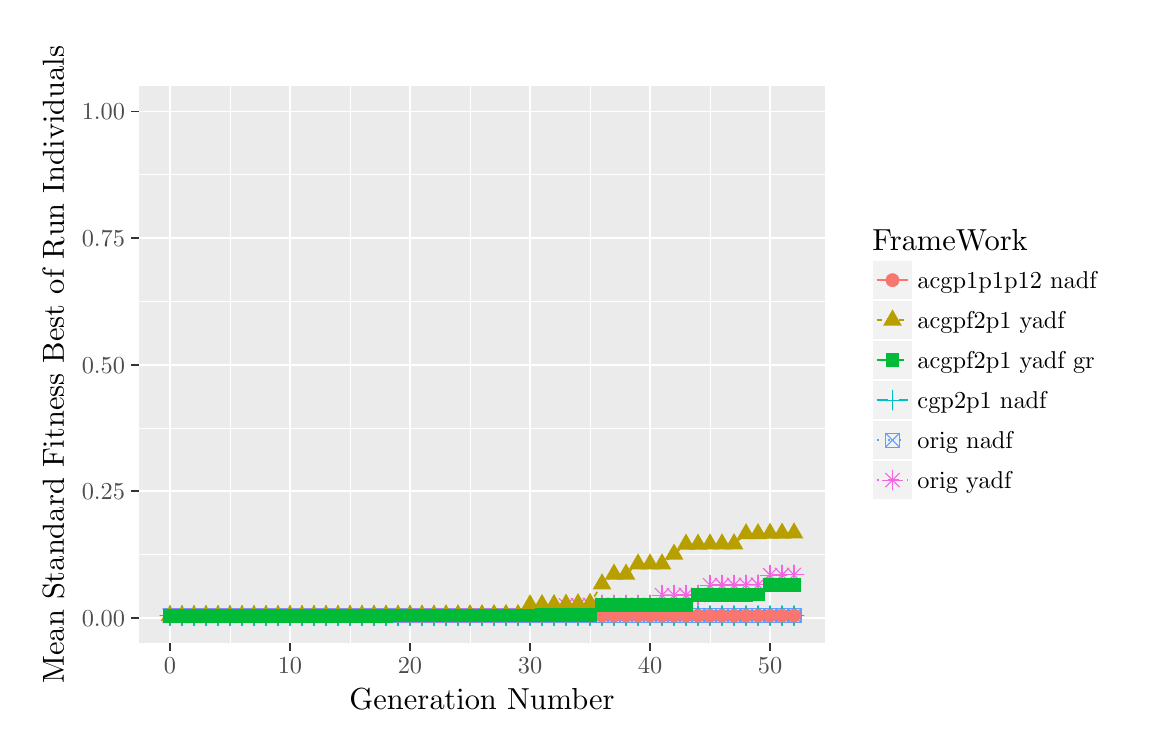
\begin{tikzpicture}[x=1pt,y=1pt]
\definecolor{fillColor}{RGB}{255,255,255}
\path[use as bounding box,fill=fillColor,fill opacity=0.00] (0,0) rectangle (397.48,252.94);
\begin{scope}
\path[clip] (  0.00,  0.00) rectangle (397.48,252.94);
\definecolor{drawColor}{RGB}{255,255,255}
\definecolor{fillColor}{RGB}{255,255,255}

\path[draw=drawColor,line width= 0.6pt,line join=round,line cap=round,fill=fillColor] (  0.00,  0.00) rectangle (397.48,252.95);
\end{scope}
\begin{scope}
\path[clip] ( 40.14, 30.56) rectangle (288.20,231.75);
\definecolor{fillColor}{gray}{0.92}

\path[fill=fillColor] ( 40.14, 30.56) rectangle (288.20,231.75);
\definecolor{drawColor}{RGB}{255,255,255}

\path[draw=drawColor,line width= 0.3pt,line join=round] ( 40.14, 62.57) --
	(288.20, 62.57);

\path[draw=drawColor,line width= 0.3pt,line join=round] ( 40.14,108.29) --
	(288.20,108.29);

\path[draw=drawColor,line width= 0.3pt,line join=round] ( 40.14,154.02) --
	(288.20,154.02);

\path[draw=drawColor,line width= 0.3pt,line join=round] ( 40.14,199.75) --
	(288.20,199.75);

\path[draw=drawColor,line width= 0.3pt,line join=round] ( 73.10, 30.56) --
	( 73.10,231.75);

\path[draw=drawColor,line width= 0.3pt,line join=round] (116.47, 30.56) --
	(116.47,231.75);

\path[draw=drawColor,line width= 0.3pt,line join=round] (159.83, 30.56) --
	(159.83,231.75);

\path[draw=drawColor,line width= 0.3pt,line join=round] (203.20, 30.56) --
	(203.20,231.75);

\path[draw=drawColor,line width= 0.3pt,line join=round] (246.57, 30.56) --
	(246.57,231.75);

\path[draw=drawColor,line width= 0.6pt,line join=round] ( 40.14, 39.70) --
	(288.20, 39.70);

\path[draw=drawColor,line width= 0.6pt,line join=round] ( 40.14, 85.43) --
	(288.20, 85.43);

\path[draw=drawColor,line width= 0.6pt,line join=round] ( 40.14,131.16) --
	(288.20,131.16);

\path[draw=drawColor,line width= 0.6pt,line join=round] ( 40.14,176.88) --
	(288.20,176.88);

\path[draw=drawColor,line width= 0.6pt,line join=round] ( 40.14,222.61) --
	(288.20,222.61);

\path[draw=drawColor,line width= 0.6pt,line join=round] ( 51.41, 30.56) --
	( 51.41,231.75);

\path[draw=drawColor,line width= 0.6pt,line join=round] ( 94.78, 30.56) --
	( 94.78,231.75);

\path[draw=drawColor,line width= 0.6pt,line join=round] (138.15, 30.56) --
	(138.15,231.75);

\path[draw=drawColor,line width= 0.6pt,line join=round] (181.52, 30.56) --
	(181.52,231.75);

\path[draw=drawColor,line width= 0.6pt,line join=round] (224.88, 30.56) --
	(224.88,231.75);

\path[draw=drawColor,line width= 0.6pt,line join=round] (268.25, 30.56) --
	(268.25,231.75);
\definecolor{drawColor}{RGB}{248,118,109}

\path[draw=drawColor,line width= 0.6pt,line join=round] ( 51.41, 40.44) --
	( 55.75, 40.44) --
	( 60.09, 40.44) --
	( 64.42, 40.44) --
	( 68.76, 40.44) --
	( 73.10, 40.44) --
	( 77.43, 40.44) --
	( 81.77, 40.44) --
	( 86.11, 40.44) --
	( 90.44, 40.44) --
	( 94.78, 40.44) --
	( 99.12, 40.44) --
	(103.45, 40.44) --
	(107.79, 40.44) --
	(112.13, 40.44) --
	(116.47, 40.44) --
	(120.80, 40.44) --
	(125.14, 40.45) --
	(129.48, 40.45) --
	(133.81, 40.45) --
	(138.15, 40.45) --
	(142.49, 40.45) --
	(146.82, 40.45) --
	(151.16, 40.45) --
	(155.50, 40.45) --
	(159.83, 40.45) --
	(164.17, 40.45) --
	(168.51, 40.45) --
	(172.84, 40.45) --
	(177.18, 40.45) --
	(181.52, 40.45) --
	(185.85, 40.46) --
	(190.19, 40.46) --
	(194.53, 40.46) --
	(198.86, 40.46) --
	(203.20, 40.46) --
	(207.54, 40.46) --
	(211.87, 40.46) --
	(216.21, 40.46) --
	(220.55, 40.46) --
	(224.88, 40.46) --
	(229.22, 40.46) --
	(233.56, 40.46) --
	(237.89, 40.46) --
	(242.23, 40.46) --
	(246.57, 40.46) --
	(250.90, 40.46) --
	(255.24, 40.46) --
	(259.58, 40.46) --
	(263.91, 40.47) --
	(268.25, 40.47) --
	(272.59, 40.47) --
	(276.92, 40.47);
\definecolor{drawColor}{RGB}{183,159,0}

\path[draw=drawColor,line width= 0.6pt,dash pattern=on 2pt off 2pt ,line join=round] ( 51.41, 40.44) --
	( 55.75, 40.44) --
	( 60.09, 40.45) --
	( 64.42, 40.46) --
	( 68.76, 40.46) --
	( 73.10, 40.47) --
	( 77.43, 40.47) --
	( 81.77, 40.48) --
	( 86.11, 40.49) --
	( 90.44, 40.50) --
	( 94.78, 40.50) --
	( 99.12, 40.51) --
	(103.45, 40.51) --
	(107.79, 40.53) --
	(112.13, 40.54) --
	(116.47, 40.55) --
	(120.80, 40.57) --
	(125.14, 40.58) --
	(129.48, 40.58) --
	(133.81, 40.59) --
	(138.15, 40.59) --
	(142.49, 40.61) --
	(146.82, 40.61) --
	(151.16, 40.72) --
	(155.50, 40.73) --
	(159.83, 40.74) --
	(164.17, 40.77) --
	(168.51, 40.81) --
	(172.84, 40.85) --
	(177.18, 40.86) --
	(181.52, 44.38) --
	(185.85, 44.42) --
	(190.19, 44.46) --
	(194.53, 44.58) --
	(198.86, 44.72) --
	(203.20, 44.86) --
	(207.54, 51.92) --
	(211.87, 55.45) --
	(216.21, 55.46) --
	(220.55, 59.11) --
	(224.88, 59.13) --
	(229.22, 59.13) --
	(233.56, 62.67) --
	(237.89, 66.27) --
	(242.23, 66.28) --
	(246.57, 66.34) --
	(250.90, 66.36) --
	(255.24, 66.40) --
	(259.58, 70.03) --
	(263.91, 70.06) --
	(268.25, 70.22) --
	(272.59, 70.23) --
	(276.92, 70.32);
\definecolor{drawColor}{RGB}{0,186,56}

\path[draw=drawColor,line width= 0.6pt,dash pattern=on 4pt off 2pt ,line join=round] ( 51.41, 40.44) --
	( 55.75, 40.44) --
	( 60.09, 40.44) --
	( 64.42, 40.45) --
	( 68.76, 40.45) --
	( 73.10, 40.45) --
	( 77.43, 40.45) --
	( 81.77, 40.46) --
	( 86.11, 40.46) --
	( 90.44, 40.46) --
	( 94.78, 40.47) --
	( 99.12, 40.47) --
	(103.45, 40.47) --
	(107.79, 40.48) --
	(112.13, 40.48) --
	(116.47, 40.48) --
	(120.80, 40.48) --
	(125.14, 40.49) --
	(129.48, 40.49) --
	(133.81, 40.49) --
	(138.15, 40.49) --
	(142.49, 40.50) --
	(146.82, 40.50) --
	(151.16, 40.51) --
	(155.50, 40.52) --
	(159.83, 40.52) --
	(164.17, 40.52) --
	(168.51, 40.54) --
	(172.84, 40.54) --
	(177.18, 40.54) --
	(181.52, 40.55) --
	(185.85, 40.58) --
	(190.19, 40.58) --
	(194.53, 40.65) --
	(198.86, 40.67) --
	(203.20, 40.68) --
	(207.54, 44.20) --
	(211.87, 44.20) --
	(216.21, 44.24) --
	(220.55, 44.32) --
	(224.88, 44.32) --
	(229.22, 44.33) --
	(233.56, 44.33) --
	(237.89, 44.34) --
	(242.23, 47.89) --
	(246.57, 47.90) --
	(250.90, 48.00) --
	(255.24, 48.00) --
	(259.58, 48.01) --
	(263.91, 48.12) --
	(268.25, 51.65) --
	(272.59, 51.66) --
	(276.92, 51.70);
\definecolor{drawColor}{RGB}{0,191,196}

\path[draw=drawColor,line width= 0.6pt,dash pattern=on 4pt off 4pt ,line join=round] ( 51.41, 40.44) --
	( 55.75, 40.44) --
	( 60.09, 40.44) --
	( 64.42, 40.45) --
	( 68.76, 40.45) --
	( 73.10, 40.45) --
	( 77.43, 40.45) --
	( 81.77, 40.45) --
	( 86.11, 40.45) --
	( 90.44, 40.45) --
	( 94.78, 40.45) --
	( 99.12, 40.45) --
	(103.45, 40.45) --
	(107.79, 40.45) --
	(112.13, 40.45) --
	(116.47, 40.45) --
	(120.80, 40.45) --
	(125.14, 40.46) --
	(129.48, 40.46) --
	(133.81, 40.46) --
	(138.15, 40.46) --
	(142.49, 40.46) --
	(146.82, 40.46) --
	(151.16, 40.46) --
	(155.50, 40.46) --
	(159.83, 40.46) --
	(164.17, 40.46) --
	(168.51, 40.47) --
	(172.84, 40.47) --
	(177.18, 40.47) --
	(181.52, 40.47) --
	(185.85, 40.47) --
	(190.19, 40.47) --
	(194.53, 40.47) --
	(198.86, 40.47) --
	(203.20, 40.47) --
	(207.54, 40.47) --
	(211.87, 40.48) --
	(216.21, 40.48) --
	(220.55, 40.48) --
	(224.88, 40.48) --
	(229.22, 40.48) --
	(233.56, 40.48) --
	(237.89, 40.48) --
	(242.23, 40.48) --
	(246.57, 40.48) --
	(250.90, 40.48) --
	(255.24, 40.48) --
	(259.58, 40.48) --
	(263.91, 40.48) --
	(268.25, 40.48) --
	(272.59, 40.48) --
	(276.92, 40.48);
\definecolor{drawColor}{RGB}{97,156,255}

\path[draw=drawColor,line width= 0.6pt,dash pattern=on 1pt off 3pt ,line join=round] ( 51.41, 40.44) --
	( 55.75, 40.44) --
	( 60.09, 40.44) --
	( 64.42, 40.44) --
	( 68.76, 40.44) --
	( 73.10, 40.44) --
	( 77.43, 40.44) --
	( 81.77, 40.44) --
	( 86.11, 40.44) --
	( 90.44, 40.44) --
	( 94.78, 40.44) --
	( 99.12, 40.44) --
	(103.45, 40.44) --
	(107.79, 40.44) --
	(112.13, 40.44) --
	(116.47, 40.44) --
	(120.80, 40.45) --
	(125.14, 40.45) --
	(129.48, 40.45) --
	(133.81, 40.45) --
	(138.15, 40.45) --
	(142.49, 40.45) --
	(146.82, 40.45) --
	(151.16, 40.45) --
	(155.50, 40.45) --
	(159.83, 40.45) --
	(164.17, 40.45) --
	(168.51, 40.45) --
	(172.84, 40.45) --
	(177.18, 40.45) --
	(181.52, 40.45) --
	(185.85, 40.45) --
	(190.19, 40.46) --
	(194.53, 40.46) --
	(198.86, 40.46) --
	(203.20, 40.46) --
	(207.54, 40.46) --
	(211.87, 40.46) --
	(216.21, 40.46) --
	(220.55, 40.46) --
	(224.88, 40.46) --
	(229.22, 40.46) --
	(233.56, 40.46) --
	(237.89, 40.46) --
	(242.23, 40.46) --
	(246.57, 40.46) --
	(250.90, 40.46) --
	(255.24, 40.46) --
	(259.58, 40.46) --
	(263.91, 40.46) --
	(268.25, 40.46) --
	(272.59, 40.46) --
	(276.92, 40.46);
\definecolor{drawColor}{RGB}{245,100,227}

\path[draw=drawColor,line width= 0.6pt,dash pattern=on 1pt off 3pt on 4pt off 3pt ,line join=round] ( 51.41, 40.44) --
	( 55.75, 40.44) --
	( 60.09, 40.44) --
	( 64.42, 40.45) --
	( 68.76, 40.45) --
	( 73.10, 40.45) --
	( 77.43, 40.46) --
	( 81.77, 40.46) --
	( 86.11, 40.46) --
	( 90.44, 40.47) --
	( 94.78, 40.47) --
	( 99.12, 40.47) --
	(103.45, 40.48) --
	(107.79, 40.48) --
	(112.13, 40.48) --
	(116.47, 40.48) --
	(120.80, 40.49) --
	(125.14, 40.49) --
	(129.48, 40.49) --
	(133.81, 40.50) --
	(138.15, 40.51) --
	(142.49, 40.51) --
	(146.82, 40.51) --
	(151.16, 40.51) --
	(155.50, 40.52) --
	(159.83, 40.54) --
	(164.17, 40.56) --
	(168.51, 40.59) --
	(172.84, 40.59) --
	(177.18, 40.60) --
	(181.52, 40.67) --
	(185.85, 40.69) --
	(190.19, 40.69) --
	(194.53, 44.22) --
	(198.86, 44.22) --
	(203.20, 44.32) --
	(207.54, 44.33) --
	(211.87, 44.33) --
	(216.21, 44.34) --
	(220.55, 44.35) --
	(224.88, 44.35) --
	(229.22, 47.87) --
	(233.56, 47.90) --
	(237.89, 47.93) --
	(242.23, 47.93) --
	(246.57, 51.52) --
	(250.90, 51.53) --
	(255.24, 51.53) --
	(259.58, 51.61) --
	(263.91, 51.63) --
	(268.25, 55.14) --
	(272.59, 55.19) --
	(276.92, 55.19);
\definecolor{drawColor}{RGB}{97,156,255}

\path[draw=drawColor,line width= 0.4pt,line join=round,line cap=round] ( 48.92, 37.94) rectangle ( 53.91, 42.93);

\path[draw=drawColor,line width= 0.4pt,line join=round,line cap=round] ( 48.92, 37.94) -- ( 53.91, 42.93);

\path[draw=drawColor,line width= 0.4pt,line join=round,line cap=round] ( 48.92, 42.93) -- ( 53.91, 37.94);

\path[draw=drawColor,line width= 0.4pt,line join=round,line cap=round] ( 53.25, 37.94) rectangle ( 58.25, 42.94);

\path[draw=drawColor,line width= 0.4pt,line join=round,line cap=round] ( 53.25, 37.94) -- ( 58.25, 42.94);

\path[draw=drawColor,line width= 0.4pt,line join=round,line cap=round] ( 53.25, 42.94) -- ( 58.25, 37.94);

\path[draw=drawColor,line width= 0.4pt,line join=round,line cap=round] ( 57.59, 37.94) rectangle ( 62.59, 42.94);

\path[draw=drawColor,line width= 0.4pt,line join=round,line cap=round] ( 57.59, 37.94) -- ( 62.59, 42.94);

\path[draw=drawColor,line width= 0.4pt,line join=round,line cap=round] ( 57.59, 42.94) -- ( 62.59, 37.94);

\path[draw=drawColor,line width= 0.4pt,line join=round,line cap=round] ( 61.93, 37.94) rectangle ( 66.92, 42.94);

\path[draw=drawColor,line width= 0.4pt,line join=round,line cap=round] ( 61.93, 37.94) -- ( 66.92, 42.94);

\path[draw=drawColor,line width= 0.4pt,line join=round,line cap=round] ( 61.93, 42.94) -- ( 66.92, 37.94);

\path[draw=drawColor,line width= 0.4pt,line join=round,line cap=round] ( 66.26, 37.94) rectangle ( 71.26, 42.94);

\path[draw=drawColor,line width= 0.4pt,line join=round,line cap=round] ( 66.26, 37.94) -- ( 71.26, 42.94);

\path[draw=drawColor,line width= 0.4pt,line join=round,line cap=round] ( 66.26, 42.94) -- ( 71.26, 37.94);

\path[draw=drawColor,line width= 0.4pt,line join=round,line cap=round] ( 70.60, 37.94) rectangle ( 75.60, 42.94);

\path[draw=drawColor,line width= 0.4pt,line join=round,line cap=round] ( 70.60, 37.94) -- ( 75.60, 42.94);

\path[draw=drawColor,line width= 0.4pt,line join=round,line cap=round] ( 70.60, 42.94) -- ( 75.60, 37.94);

\path[draw=drawColor,line width= 0.4pt,line join=round,line cap=round] ( 74.94, 37.94) rectangle ( 79.93, 42.94);

\path[draw=drawColor,line width= 0.4pt,line join=round,line cap=round] ( 74.94, 37.94) -- ( 79.93, 42.94);

\path[draw=drawColor,line width= 0.4pt,line join=round,line cap=round] ( 74.94, 42.94) -- ( 79.93, 37.94);

\path[draw=drawColor,line width= 0.4pt,line join=round,line cap=round] ( 79.27, 37.94) rectangle ( 84.27, 42.94);

\path[draw=drawColor,line width= 0.4pt,line join=round,line cap=round] ( 79.27, 37.94) -- ( 84.27, 42.94);

\path[draw=drawColor,line width= 0.4pt,line join=round,line cap=round] ( 79.27, 42.94) -- ( 84.27, 37.94);

\path[draw=drawColor,line width= 0.4pt,line join=round,line cap=round] ( 83.61, 37.94) rectangle ( 88.61, 42.94);

\path[draw=drawColor,line width= 0.4pt,line join=round,line cap=round] ( 83.61, 37.94) -- ( 88.61, 42.94);

\path[draw=drawColor,line width= 0.4pt,line join=round,line cap=round] ( 83.61, 42.94) -- ( 88.61, 37.94);

\path[draw=drawColor,line width= 0.4pt,line join=round,line cap=round] ( 87.95, 37.95) rectangle ( 92.94, 42.94);

\path[draw=drawColor,line width= 0.4pt,line join=round,line cap=round] ( 87.95, 37.95) -- ( 92.94, 42.94);

\path[draw=drawColor,line width= 0.4pt,line join=round,line cap=round] ( 87.95, 42.94) -- ( 92.94, 37.95);

\path[draw=drawColor,line width= 0.4pt,line join=round,line cap=round] ( 92.28, 37.95) rectangle ( 97.28, 42.94);

\path[draw=drawColor,line width= 0.4pt,line join=round,line cap=round] ( 92.28, 37.95) -- ( 97.28, 42.94);

\path[draw=drawColor,line width= 0.4pt,line join=round,line cap=round] ( 92.28, 42.94) -- ( 97.28, 37.95);

\path[draw=drawColor,line width= 0.4pt,line join=round,line cap=round] ( 96.62, 37.95) rectangle (101.62, 42.94);

\path[draw=drawColor,line width= 0.4pt,line join=round,line cap=round] ( 96.62, 37.95) -- (101.62, 42.94);

\path[draw=drawColor,line width= 0.4pt,line join=round,line cap=round] ( 96.62, 42.94) -- (101.62, 37.95);

\path[draw=drawColor,line width= 0.4pt,line join=round,line cap=round] (100.96, 37.95) rectangle (105.95, 42.94);

\path[draw=drawColor,line width= 0.4pt,line join=round,line cap=round] (100.96, 37.95) -- (105.95, 42.94);

\path[draw=drawColor,line width= 0.4pt,line join=round,line cap=round] (100.96, 42.94) -- (105.95, 37.95);

\path[draw=drawColor,line width= 0.4pt,line join=round,line cap=round] (105.29, 37.95) rectangle (110.29, 42.94);

\path[draw=drawColor,line width= 0.4pt,line join=round,line cap=round] (105.29, 37.95) -- (110.29, 42.94);

\path[draw=drawColor,line width= 0.4pt,line join=round,line cap=round] (105.29, 42.94) -- (110.29, 37.95);

\path[draw=drawColor,line width= 0.4pt,line join=round,line cap=round] (109.63, 37.95) rectangle (114.63, 42.94);

\path[draw=drawColor,line width= 0.4pt,line join=round,line cap=round] (109.63, 37.95) -- (114.63, 42.94);

\path[draw=drawColor,line width= 0.4pt,line join=round,line cap=round] (109.63, 42.94) -- (114.63, 37.95);

\path[draw=drawColor,line width= 0.4pt,line join=round,line cap=round] (113.97, 37.95) rectangle (118.96, 42.94);

\path[draw=drawColor,line width= 0.4pt,line join=round,line cap=round] (113.97, 37.95) -- (118.96, 42.94);

\path[draw=drawColor,line width= 0.4pt,line join=round,line cap=round] (113.97, 42.94) -- (118.96, 37.95);

\path[draw=drawColor,line width= 0.4pt,line join=round,line cap=round] (118.30, 37.95) rectangle (123.30, 42.94);

\path[draw=drawColor,line width= 0.4pt,line join=round,line cap=round] (118.30, 37.95) -- (123.30, 42.94);

\path[draw=drawColor,line width= 0.4pt,line join=round,line cap=round] (118.30, 42.94) -- (123.30, 37.95);

\path[draw=drawColor,line width= 0.4pt,line join=round,line cap=round] (122.64, 37.95) rectangle (127.64, 42.94);

\path[draw=drawColor,line width= 0.4pt,line join=round,line cap=round] (122.64, 37.95) -- (127.64, 42.94);

\path[draw=drawColor,line width= 0.4pt,line join=round,line cap=round] (122.64, 42.94) -- (127.64, 37.95);

\path[draw=drawColor,line width= 0.4pt,line join=round,line cap=round] (126.98, 37.95) rectangle (131.97, 42.95);

\path[draw=drawColor,line width= 0.4pt,line join=round,line cap=round] (126.98, 37.95) -- (131.97, 42.95);

\path[draw=drawColor,line width= 0.4pt,line join=round,line cap=round] (126.98, 42.95) -- (131.97, 37.95);

\path[draw=drawColor,line width= 0.4pt,line join=round,line cap=round] (131.31, 37.95) rectangle (136.31, 42.95);

\path[draw=drawColor,line width= 0.4pt,line join=round,line cap=round] (131.31, 37.95) -- (136.31, 42.95);

\path[draw=drawColor,line width= 0.4pt,line join=round,line cap=round] (131.31, 42.95) -- (136.31, 37.95);

\path[draw=drawColor,line width= 0.4pt,line join=round,line cap=round] (135.65, 37.95) rectangle (140.65, 42.95);

\path[draw=drawColor,line width= 0.4pt,line join=round,line cap=round] (135.65, 37.95) -- (140.65, 42.95);

\path[draw=drawColor,line width= 0.4pt,line join=round,line cap=round] (135.65, 42.95) -- (140.65, 37.95);

\path[draw=drawColor,line width= 0.4pt,line join=round,line cap=round] (139.99, 37.95) rectangle (144.98, 42.95);

\path[draw=drawColor,line width= 0.4pt,line join=round,line cap=round] (139.99, 37.95) -- (144.98, 42.95);

\path[draw=drawColor,line width= 0.4pt,line join=round,line cap=round] (139.99, 42.95) -- (144.98, 37.95);

\path[draw=drawColor,line width= 0.4pt,line join=round,line cap=round] (144.32, 37.96) rectangle (149.32, 42.95);

\path[draw=drawColor,line width= 0.4pt,line join=round,line cap=round] (144.32, 37.96) -- (149.32, 42.95);

\path[draw=drawColor,line width= 0.4pt,line join=round,line cap=round] (144.32, 42.95) -- (149.32, 37.96);

\path[draw=drawColor,line width= 0.4pt,line join=round,line cap=round] (148.66, 37.96) rectangle (153.66, 42.95);

\path[draw=drawColor,line width= 0.4pt,line join=round,line cap=round] (148.66, 37.96) -- (153.66, 42.95);

\path[draw=drawColor,line width= 0.4pt,line join=round,line cap=round] (148.66, 42.95) -- (153.66, 37.96);

\path[draw=drawColor,line width= 0.4pt,line join=round,line cap=round] (153.00, 37.96) rectangle (157.99, 42.95);

\path[draw=drawColor,line width= 0.4pt,line join=round,line cap=round] (153.00, 37.96) -- (157.99, 42.95);

\path[draw=drawColor,line width= 0.4pt,line join=round,line cap=round] (153.00, 42.95) -- (157.99, 37.96);

\path[draw=drawColor,line width= 0.4pt,line join=round,line cap=round] (157.33, 37.96) rectangle (162.33, 42.95);

\path[draw=drawColor,line width= 0.4pt,line join=round,line cap=round] (157.33, 37.96) -- (162.33, 42.95);

\path[draw=drawColor,line width= 0.4pt,line join=round,line cap=round] (157.33, 42.95) -- (162.33, 37.96);

\path[draw=drawColor,line width= 0.4pt,line join=round,line cap=round] (161.67, 37.96) rectangle (166.67, 42.95);

\path[draw=drawColor,line width= 0.4pt,line join=round,line cap=round] (161.67, 37.96) -- (166.67, 42.95);

\path[draw=drawColor,line width= 0.4pt,line join=round,line cap=round] (161.67, 42.95) -- (166.67, 37.96);

\path[draw=drawColor,line width= 0.4pt,line join=round,line cap=round] (166.01, 37.96) rectangle (171.00, 42.95);

\path[draw=drawColor,line width= 0.4pt,line join=round,line cap=round] (166.01, 37.96) -- (171.00, 42.95);

\path[draw=drawColor,line width= 0.4pt,line join=round,line cap=round] (166.01, 42.95) -- (171.00, 37.96);

\path[draw=drawColor,line width= 0.4pt,line join=round,line cap=round] (170.35, 37.96) rectangle (175.34, 42.95);

\path[draw=drawColor,line width= 0.4pt,line join=round,line cap=round] (170.35, 37.96) -- (175.34, 42.95);

\path[draw=drawColor,line width= 0.4pt,line join=round,line cap=round] (170.35, 42.95) -- (175.34, 37.96);

\path[draw=drawColor,line width= 0.4pt,line join=round,line cap=round] (174.68, 37.96) rectangle (179.68, 42.95);

\path[draw=drawColor,line width= 0.4pt,line join=round,line cap=round] (174.68, 37.96) -- (179.68, 42.95);

\path[draw=drawColor,line width= 0.4pt,line join=round,line cap=round] (174.68, 42.95) -- (179.68, 37.96);

\path[draw=drawColor,line width= 0.4pt,line join=round,line cap=round] (179.02, 37.96) rectangle (184.01, 42.95);

\path[draw=drawColor,line width= 0.4pt,line join=round,line cap=round] (179.02, 37.96) -- (184.01, 42.95);

\path[draw=drawColor,line width= 0.4pt,line join=round,line cap=round] (179.02, 42.95) -- (184.01, 37.96);

\path[draw=drawColor,line width= 0.4pt,line join=round,line cap=round] (183.36, 37.96) rectangle (188.35, 42.95);

\path[draw=drawColor,line width= 0.4pt,line join=round,line cap=round] (183.36, 37.96) -- (188.35, 42.95);

\path[draw=drawColor,line width= 0.4pt,line join=round,line cap=round] (183.36, 42.95) -- (188.35, 37.96);

\path[draw=drawColor,line width= 0.4pt,line join=round,line cap=round] (187.69, 37.96) rectangle (192.69, 42.95);

\path[draw=drawColor,line width= 0.4pt,line join=round,line cap=round] (187.69, 37.96) -- (192.69, 42.95);

\path[draw=drawColor,line width= 0.4pt,line join=round,line cap=round] (187.69, 42.95) -- (192.69, 37.96);

\path[draw=drawColor,line width= 0.4pt,line join=round,line cap=round] (192.03, 37.96) rectangle (197.02, 42.95);

\path[draw=drawColor,line width= 0.4pt,line join=round,line cap=round] (192.03, 37.96) -- (197.02, 42.95);

\path[draw=drawColor,line width= 0.4pt,line join=round,line cap=round] (192.03, 42.95) -- (197.02, 37.96);

\path[draw=drawColor,line width= 0.4pt,line join=round,line cap=round] (196.37, 37.96) rectangle (201.36, 42.95);

\path[draw=drawColor,line width= 0.4pt,line join=round,line cap=round] (196.37, 37.96) -- (201.36, 42.95);

\path[draw=drawColor,line width= 0.4pt,line join=round,line cap=round] (196.37, 42.95) -- (201.36, 37.96);

\path[draw=drawColor,line width= 0.4pt,line join=round,line cap=round] (200.70, 37.96) rectangle (205.70, 42.95);

\path[draw=drawColor,line width= 0.4pt,line join=round,line cap=round] (200.70, 37.96) -- (205.70, 42.95);

\path[draw=drawColor,line width= 0.4pt,line join=round,line cap=round] (200.70, 42.95) -- (205.70, 37.96);

\path[draw=drawColor,line width= 0.4pt,line join=round,line cap=round] (205.04, 37.96) rectangle (210.03, 42.95);

\path[draw=drawColor,line width= 0.4pt,line join=round,line cap=round] (205.04, 37.96) -- (210.03, 42.95);

\path[draw=drawColor,line width= 0.4pt,line join=round,line cap=round] (205.04, 42.95) -- (210.03, 37.96);

\path[draw=drawColor,line width= 0.4pt,line join=round,line cap=round] (209.38, 37.96) rectangle (214.37, 42.95);

\path[draw=drawColor,line width= 0.4pt,line join=round,line cap=round] (209.38, 37.96) -- (214.37, 42.95);

\path[draw=drawColor,line width= 0.4pt,line join=round,line cap=round] (209.38, 42.95) -- (214.37, 37.96);

\path[draw=drawColor,line width= 0.4pt,line join=round,line cap=round] (213.71, 37.96) rectangle (218.71, 42.95);

\path[draw=drawColor,line width= 0.4pt,line join=round,line cap=round] (213.71, 37.96) -- (218.71, 42.95);

\path[draw=drawColor,line width= 0.4pt,line join=round,line cap=round] (213.71, 42.95) -- (218.71, 37.96);

\path[draw=drawColor,line width= 0.4pt,line join=round,line cap=round] (218.05, 37.96) rectangle (223.04, 42.96);

\path[draw=drawColor,line width= 0.4pt,line join=round,line cap=round] (218.05, 37.96) -- (223.04, 42.96);

\path[draw=drawColor,line width= 0.4pt,line join=round,line cap=round] (218.05, 42.96) -- (223.04, 37.96);

\path[draw=drawColor,line width= 0.4pt,line join=round,line cap=round] (222.39, 37.96) rectangle (227.38, 42.96);

\path[draw=drawColor,line width= 0.4pt,line join=round,line cap=round] (222.39, 37.96) -- (227.38, 42.96);

\path[draw=drawColor,line width= 0.4pt,line join=round,line cap=round] (222.39, 42.96) -- (227.38, 37.96);

\path[draw=drawColor,line width= 0.4pt,line join=round,line cap=round] (226.72, 37.96) rectangle (231.72, 42.96);

\path[draw=drawColor,line width= 0.4pt,line join=round,line cap=round] (226.72, 37.96) -- (231.72, 42.96);

\path[draw=drawColor,line width= 0.4pt,line join=round,line cap=round] (226.72, 42.96) -- (231.72, 37.96);

\path[draw=drawColor,line width= 0.4pt,line join=round,line cap=round] (231.06, 37.96) rectangle (236.05, 42.96);

\path[draw=drawColor,line width= 0.4pt,line join=round,line cap=round] (231.06, 37.96) -- (236.05, 42.96);

\path[draw=drawColor,line width= 0.4pt,line join=round,line cap=round] (231.06, 42.96) -- (236.05, 37.96);

\path[draw=drawColor,line width= 0.4pt,line join=round,line cap=round] (235.40, 37.96) rectangle (240.39, 42.96);

\path[draw=drawColor,line width= 0.4pt,line join=round,line cap=round] (235.40, 37.96) -- (240.39, 42.96);

\path[draw=drawColor,line width= 0.4pt,line join=round,line cap=round] (235.40, 42.96) -- (240.39, 37.96);

\path[draw=drawColor,line width= 0.4pt,line join=round,line cap=round] (239.73, 37.96) rectangle (244.73, 42.96);

\path[draw=drawColor,line width= 0.4pt,line join=round,line cap=round] (239.73, 37.96) -- (244.73, 42.96);

\path[draw=drawColor,line width= 0.4pt,line join=round,line cap=round] (239.73, 42.96) -- (244.73, 37.96);

\path[draw=drawColor,line width= 0.4pt,line join=round,line cap=round] (244.07, 37.96) rectangle (249.06, 42.96);

\path[draw=drawColor,line width= 0.4pt,line join=round,line cap=round] (244.07, 37.96) -- (249.06, 42.96);

\path[draw=drawColor,line width= 0.4pt,line join=round,line cap=round] (244.07, 42.96) -- (249.06, 37.96);

\path[draw=drawColor,line width= 0.4pt,line join=round,line cap=round] (248.41, 37.96) rectangle (253.40, 42.96);

\path[draw=drawColor,line width= 0.4pt,line join=round,line cap=round] (248.41, 37.96) -- (253.40, 42.96);

\path[draw=drawColor,line width= 0.4pt,line join=round,line cap=round] (248.41, 42.96) -- (253.40, 37.96);

\path[draw=drawColor,line width= 0.4pt,line join=round,line cap=round] (252.74, 37.96) rectangle (257.74, 42.96);

\path[draw=drawColor,line width= 0.4pt,line join=round,line cap=round] (252.74, 37.96) -- (257.74, 42.96);

\path[draw=drawColor,line width= 0.4pt,line join=round,line cap=round] (252.74, 42.96) -- (257.74, 37.96);

\path[draw=drawColor,line width= 0.4pt,line join=round,line cap=round] (257.08, 37.96) rectangle (262.07, 42.96);

\path[draw=drawColor,line width= 0.4pt,line join=round,line cap=round] (257.08, 37.96) -- (262.07, 42.96);

\path[draw=drawColor,line width= 0.4pt,line join=round,line cap=round] (257.08, 42.96) -- (262.07, 37.96);

\path[draw=drawColor,line width= 0.4pt,line join=round,line cap=round] (261.42, 37.96) rectangle (266.41, 42.96);

\path[draw=drawColor,line width= 0.4pt,line join=round,line cap=round] (261.42, 37.96) -- (266.41, 42.96);

\path[draw=drawColor,line width= 0.4pt,line join=round,line cap=round] (261.42, 42.96) -- (266.41, 37.96);

\path[draw=drawColor,line width= 0.4pt,line join=round,line cap=round] (265.75, 37.96) rectangle (270.75, 42.96);

\path[draw=drawColor,line width= 0.4pt,line join=round,line cap=round] (265.75, 37.96) -- (270.75, 42.96);

\path[draw=drawColor,line width= 0.4pt,line join=round,line cap=round] (265.75, 42.96) -- (270.75, 37.96);

\path[draw=drawColor,line width= 0.4pt,line join=round,line cap=round] (270.09, 37.96) rectangle (275.09, 42.96);

\path[draw=drawColor,line width= 0.4pt,line join=round,line cap=round] (270.09, 37.96) -- (275.09, 42.96);

\path[draw=drawColor,line width= 0.4pt,line join=round,line cap=round] (270.09, 42.96) -- (275.09, 37.96);

\path[draw=drawColor,line width= 0.4pt,line join=round,line cap=round] (274.43, 37.96) rectangle (279.42, 42.96);

\path[draw=drawColor,line width= 0.4pt,line join=round,line cap=round] (274.43, 37.96) -- (279.42, 42.96);

\path[draw=drawColor,line width= 0.4pt,line join=round,line cap=round] (274.43, 42.96) -- (279.42, 37.96);
\definecolor{drawColor}{RGB}{245,100,227}

\path[draw=drawColor,line width= 0.4pt,line join=round,line cap=round] ( 48.92, 37.94) -- ( 53.91, 42.93);

\path[draw=drawColor,line width= 0.4pt,line join=round,line cap=round] ( 48.92, 42.93) -- ( 53.91, 37.94);

\path[draw=drawColor,line width= 0.4pt,line join=round,line cap=round] ( 47.88, 40.44) -- ( 54.95, 40.44);

\path[draw=drawColor,line width= 0.4pt,line join=round,line cap=round] ( 51.41, 36.90) -- ( 51.41, 43.97);

\path[draw=drawColor,line width= 0.4pt,line join=round,line cap=round] ( 53.25, 37.94) -- ( 58.25, 42.93);

\path[draw=drawColor,line width= 0.4pt,line join=round,line cap=round] ( 53.25, 42.93) -- ( 58.25, 37.94);

\path[draw=drawColor,line width= 0.4pt,line join=round,line cap=round] ( 52.22, 40.44) -- ( 59.28, 40.44);

\path[draw=drawColor,line width= 0.4pt,line join=round,line cap=round] ( 55.75, 36.90) -- ( 55.75, 43.97);

\path[draw=drawColor,line width= 0.4pt,line join=round,line cap=round] ( 57.59, 37.94) -- ( 62.59, 42.94);

\path[draw=drawColor,line width= 0.4pt,line join=round,line cap=round] ( 57.59, 42.94) -- ( 62.59, 37.94);

\path[draw=drawColor,line width= 0.4pt,line join=round,line cap=round] ( 56.56, 40.44) -- ( 63.62, 40.44);

\path[draw=drawColor,line width= 0.4pt,line join=round,line cap=round] ( 60.09, 36.91) -- ( 60.09, 43.97);

\path[draw=drawColor,line width= 0.4pt,line join=round,line cap=round] ( 61.93, 37.95) -- ( 66.92, 42.94);

\path[draw=drawColor,line width= 0.4pt,line join=round,line cap=round] ( 61.93, 42.94) -- ( 66.92, 37.95);

\path[draw=drawColor,line width= 0.4pt,line join=round,line cap=round] ( 60.89, 40.45) -- ( 67.96, 40.45);

\path[draw=drawColor,line width= 0.4pt,line join=round,line cap=round] ( 64.42, 36.91) -- ( 64.42, 43.98);

\path[draw=drawColor,line width= 0.4pt,line join=round,line cap=round] ( 66.26, 37.95) -- ( 71.26, 42.95);

\path[draw=drawColor,line width= 0.4pt,line join=round,line cap=round] ( 66.26, 42.95) -- ( 71.26, 37.95);

\path[draw=drawColor,line width= 0.4pt,line join=round,line cap=round] ( 65.23, 40.45) -- ( 72.29, 40.45);

\path[draw=drawColor,line width= 0.4pt,line join=round,line cap=round] ( 68.76, 36.92) -- ( 68.76, 43.98);

\path[draw=drawColor,line width= 0.4pt,line join=round,line cap=round] ( 70.60, 37.96) -- ( 75.60, 42.95);

\path[draw=drawColor,line width= 0.4pt,line join=round,line cap=round] ( 70.60, 42.95) -- ( 75.60, 37.96);

\path[draw=drawColor,line width= 0.4pt,line join=round,line cap=round] ( 69.57, 40.45) -- ( 76.63, 40.45);

\path[draw=drawColor,line width= 0.4pt,line join=round,line cap=round] ( 73.10, 36.92) -- ( 73.10, 43.99);

\path[draw=drawColor,line width= 0.4pt,line join=round,line cap=round] ( 74.94, 37.96) -- ( 79.93, 42.96);

\path[draw=drawColor,line width= 0.4pt,line join=round,line cap=round] ( 74.94, 42.96) -- ( 79.93, 37.96);

\path[draw=drawColor,line width= 0.4pt,line join=round,line cap=round] ( 73.90, 40.46) -- ( 80.97, 40.46);

\path[draw=drawColor,line width= 0.4pt,line join=round,line cap=round] ( 77.43, 36.93) -- ( 77.43, 43.99);

\path[draw=drawColor,line width= 0.4pt,line join=round,line cap=round] ( 79.27, 37.96) -- ( 84.27, 42.96);

\path[draw=drawColor,line width= 0.4pt,line join=round,line cap=round] ( 79.27, 42.96) -- ( 84.27, 37.96);

\path[draw=drawColor,line width= 0.4pt,line join=round,line cap=round] ( 78.24, 40.46) -- ( 85.30, 40.46);

\path[draw=drawColor,line width= 0.4pt,line join=round,line cap=round] ( 81.77, 36.93) -- ( 81.77, 43.99);

\path[draw=drawColor,line width= 0.4pt,line join=round,line cap=round] ( 83.61, 37.97) -- ( 88.61, 42.96);

\path[draw=drawColor,line width= 0.4pt,line join=round,line cap=round] ( 83.61, 42.96) -- ( 88.61, 37.97);

\path[draw=drawColor,line width= 0.4pt,line join=round,line cap=round] ( 82.58, 40.46) -- ( 89.64, 40.46);

\path[draw=drawColor,line width= 0.4pt,line join=round,line cap=round] ( 86.11, 36.93) -- ( 86.11, 44.00);

\path[draw=drawColor,line width= 0.4pt,line join=round,line cap=round] ( 87.95, 37.97) -- ( 92.94, 42.96);

\path[draw=drawColor,line width= 0.4pt,line join=round,line cap=round] ( 87.95, 42.96) -- ( 92.94, 37.97);

\path[draw=drawColor,line width= 0.4pt,line join=round,line cap=round] ( 86.91, 40.47) -- ( 93.98, 40.47);

\path[draw=drawColor,line width= 0.4pt,line join=round,line cap=round] ( 90.44, 36.93) -- ( 90.44, 44.00);

\path[draw=drawColor,line width= 0.4pt,line join=round,line cap=round] ( 92.28, 37.97) -- ( 97.28, 42.97);

\path[draw=drawColor,line width= 0.4pt,line join=round,line cap=round] ( 92.28, 42.97) -- ( 97.28, 37.97);

\path[draw=drawColor,line width= 0.4pt,line join=round,line cap=round] ( 91.25, 40.47) -- ( 98.31, 40.47);

\path[draw=drawColor,line width= 0.4pt,line join=round,line cap=round] ( 94.78, 36.94) -- ( 94.78, 44.00);

\path[draw=drawColor,line width= 0.4pt,line join=round,line cap=round] ( 96.62, 37.97) -- (101.62, 42.97);

\path[draw=drawColor,line width= 0.4pt,line join=round,line cap=round] ( 96.62, 42.97) -- (101.62, 37.97);

\path[draw=drawColor,line width= 0.4pt,line join=round,line cap=round] ( 95.59, 40.47) -- (102.65, 40.47);

\path[draw=drawColor,line width= 0.4pt,line join=round,line cap=round] ( 99.12, 36.94) -- ( 99.12, 44.00);

\path[draw=drawColor,line width= 0.4pt,line join=round,line cap=round] (100.96, 37.98) -- (105.95, 42.97);

\path[draw=drawColor,line width= 0.4pt,line join=round,line cap=round] (100.96, 42.97) -- (105.95, 37.98);

\path[draw=drawColor,line width= 0.4pt,line join=round,line cap=round] ( 99.92, 40.48) -- (106.99, 40.48);

\path[draw=drawColor,line width= 0.4pt,line join=round,line cap=round] (103.45, 36.94) -- (103.45, 44.01);

\path[draw=drawColor,line width= 0.4pt,line join=round,line cap=round] (105.29, 37.98) -- (110.29, 42.97);

\path[draw=drawColor,line width= 0.4pt,line join=round,line cap=round] (105.29, 42.97) -- (110.29, 37.98);

\path[draw=drawColor,line width= 0.4pt,line join=round,line cap=round] (104.26, 40.48) -- (111.32, 40.48);

\path[draw=drawColor,line width= 0.4pt,line join=round,line cap=round] (107.79, 36.94) -- (107.79, 44.01);

\path[draw=drawColor,line width= 0.4pt,line join=round,line cap=round] (109.63, 37.98) -- (114.63, 42.98);

\path[draw=drawColor,line width= 0.4pt,line join=round,line cap=round] (109.63, 42.98) -- (114.63, 37.98);

\path[draw=drawColor,line width= 0.4pt,line join=round,line cap=round] (108.60, 40.48) -- (115.66, 40.48);

\path[draw=drawColor,line width= 0.4pt,line join=round,line cap=round] (112.13, 36.95) -- (112.13, 44.01);

\path[draw=drawColor,line width= 0.4pt,line join=round,line cap=round] (113.97, 37.98) -- (118.96, 42.98);

\path[draw=drawColor,line width= 0.4pt,line join=round,line cap=round] (113.97, 42.98) -- (118.96, 37.98);

\path[draw=drawColor,line width= 0.4pt,line join=round,line cap=round] (112.93, 40.48) -- (120.00, 40.48);

\path[draw=drawColor,line width= 0.4pt,line join=round,line cap=round] (116.47, 36.95) -- (116.47, 44.01);

\path[draw=drawColor,line width= 0.4pt,line join=round,line cap=round] (118.30, 37.99) -- (123.30, 42.99);

\path[draw=drawColor,line width= 0.4pt,line join=round,line cap=round] (118.30, 42.99) -- (123.30, 37.99);

\path[draw=drawColor,line width= 0.4pt,line join=round,line cap=round] (117.27, 40.49) -- (124.33, 40.49);

\path[draw=drawColor,line width= 0.4pt,line join=round,line cap=round] (120.80, 36.96) -- (120.80, 44.02);

\path[draw=drawColor,line width= 0.4pt,line join=round,line cap=round] (122.64, 37.99) -- (127.64, 42.99);

\path[draw=drawColor,line width= 0.4pt,line join=round,line cap=round] (122.64, 42.99) -- (127.64, 37.99);

\path[draw=drawColor,line width= 0.4pt,line join=round,line cap=round] (121.61, 40.49) -- (128.67, 40.49);

\path[draw=drawColor,line width= 0.4pt,line join=round,line cap=round] (125.14, 36.96) -- (125.14, 44.02);

\path[draw=drawColor,line width= 0.4pt,line join=round,line cap=round] (126.98, 37.99) -- (131.97, 42.99);

\path[draw=drawColor,line width= 0.4pt,line join=round,line cap=round] (126.98, 42.99) -- (131.97, 37.99);

\path[draw=drawColor,line width= 0.4pt,line join=round,line cap=round] (125.94, 40.49) -- (133.01, 40.49);

\path[draw=drawColor,line width= 0.4pt,line join=round,line cap=round] (129.48, 36.96) -- (129.48, 44.02);

\path[draw=drawColor,line width= 0.4pt,line join=round,line cap=round] (131.31, 38.00) -- (136.31, 42.99);

\path[draw=drawColor,line width= 0.4pt,line join=round,line cap=round] (131.31, 42.99) -- (136.31, 38.00);

\path[draw=drawColor,line width= 0.4pt,line join=round,line cap=round] (130.28, 40.50) -- (137.34, 40.50);

\path[draw=drawColor,line width= 0.4pt,line join=round,line cap=round] (133.81, 36.96) -- (133.81, 44.03);

\path[draw=drawColor,line width= 0.4pt,line join=round,line cap=round] (135.65, 38.01) -- (140.65, 43.01);

\path[draw=drawColor,line width= 0.4pt,line join=round,line cap=round] (135.65, 43.01) -- (140.65, 38.01);

\path[draw=drawColor,line width= 0.4pt,line join=round,line cap=round] (134.62, 40.51) -- (141.68, 40.51);

\path[draw=drawColor,line width= 0.4pt,line join=round,line cap=round] (138.15, 36.98) -- (138.15, 44.04);

\path[draw=drawColor,line width= 0.4pt,line join=round,line cap=round] (139.99, 38.01) -- (144.98, 43.01);

\path[draw=drawColor,line width= 0.4pt,line join=round,line cap=round] (139.99, 43.01) -- (144.98, 38.01);

\path[draw=drawColor,line width= 0.4pt,line join=round,line cap=round] (138.95, 40.51) -- (146.02, 40.51);

\path[draw=drawColor,line width= 0.4pt,line join=round,line cap=round] (142.49, 36.98) -- (142.49, 44.04);

\path[draw=drawColor,line width= 0.4pt,line join=round,line cap=round] (144.32, 38.01) -- (149.32, 43.01);

\path[draw=drawColor,line width= 0.4pt,line join=round,line cap=round] (144.32, 43.01) -- (149.32, 38.01);

\path[draw=drawColor,line width= 0.4pt,line join=round,line cap=round] (143.29, 40.51) -- (150.35, 40.51);

\path[draw=drawColor,line width= 0.4pt,line join=round,line cap=round] (146.82, 36.98) -- (146.82, 44.04);

\path[draw=drawColor,line width= 0.4pt,line join=round,line cap=round] (148.66, 38.01) -- (153.66, 43.01);

\path[draw=drawColor,line width= 0.4pt,line join=round,line cap=round] (148.66, 43.01) -- (153.66, 38.01);

\path[draw=drawColor,line width= 0.4pt,line join=round,line cap=round] (147.63, 40.51) -- (154.69, 40.51);

\path[draw=drawColor,line width= 0.4pt,line join=round,line cap=round] (151.16, 36.98) -- (151.16, 44.04);

\path[draw=drawColor,line width= 0.4pt,line join=round,line cap=round] (153.00, 38.03) -- (157.99, 43.02);

\path[draw=drawColor,line width= 0.4pt,line join=round,line cap=round] (153.00, 43.02) -- (157.99, 38.03);

\path[draw=drawColor,line width= 0.4pt,line join=round,line cap=round] (151.96, 40.52) -- (159.03, 40.52);

\path[draw=drawColor,line width= 0.4pt,line join=round,line cap=round] (155.50, 36.99) -- (155.50, 44.06);

\path[draw=drawColor,line width= 0.4pt,line join=round,line cap=round] (157.33, 38.04) -- (162.33, 43.04);

\path[draw=drawColor,line width= 0.4pt,line join=round,line cap=round] (157.33, 43.04) -- (162.33, 38.04);

\path[draw=drawColor,line width= 0.4pt,line join=round,line cap=round] (156.30, 40.54) -- (163.36, 40.54);

\path[draw=drawColor,line width= 0.4pt,line join=round,line cap=round] (159.83, 37.01) -- (159.83, 44.07);

\path[draw=drawColor,line width= 0.4pt,line join=round,line cap=round] (161.67, 38.06) -- (166.67, 43.05);

\path[draw=drawColor,line width= 0.4pt,line join=round,line cap=round] (161.67, 43.05) -- (166.67, 38.06);

\path[draw=drawColor,line width= 0.4pt,line join=round,line cap=round] (160.64, 40.56) -- (167.70, 40.56);

\path[draw=drawColor,line width= 0.4pt,line join=round,line cap=round] (164.17, 37.02) -- (164.17, 44.09);

\path[draw=drawColor,line width= 0.4pt,line join=round,line cap=round] (166.01, 38.10) -- (171.00, 43.09);

\path[draw=drawColor,line width= 0.4pt,line join=round,line cap=round] (166.01, 43.09) -- (171.00, 38.10);

\path[draw=drawColor,line width= 0.4pt,line join=round,line cap=round] (164.97, 40.59) -- (172.04, 40.59);

\path[draw=drawColor,line width= 0.4pt,line join=round,line cap=round] (168.51, 37.06) -- (168.51, 44.13);

\path[draw=drawColor,line width= 0.4pt,line join=round,line cap=round] (170.35, 38.10) -- (175.34, 43.09);

\path[draw=drawColor,line width= 0.4pt,line join=round,line cap=round] (170.35, 43.09) -- (175.34, 38.10);

\path[draw=drawColor,line width= 0.4pt,line join=round,line cap=round] (169.31, 40.59) -- (176.37, 40.59);

\path[draw=drawColor,line width= 0.4pt,line join=round,line cap=round] (172.84, 37.06) -- (172.84, 44.13);

\path[draw=drawColor,line width= 0.4pt,line join=round,line cap=round] (174.68, 38.10) -- (179.68, 43.09);

\path[draw=drawColor,line width= 0.4pt,line join=round,line cap=round] (174.68, 43.09) -- (179.68, 38.10);

\path[draw=drawColor,line width= 0.4pt,line join=round,line cap=round] (173.65, 40.60) -- (180.71, 40.60);

\path[draw=drawColor,line width= 0.4pt,line join=round,line cap=round] (177.18, 37.06) -- (177.18, 44.13);

\path[draw=drawColor,line width= 0.4pt,line join=round,line cap=round] (179.02, 38.18) -- (184.01, 43.17);

\path[draw=drawColor,line width= 0.4pt,line join=round,line cap=round] (179.02, 43.17) -- (184.01, 38.18);

\path[draw=drawColor,line width= 0.4pt,line join=round,line cap=round] (177.98, 40.67) -- (185.05, 40.67);

\path[draw=drawColor,line width= 0.4pt,line join=round,line cap=round] (181.52, 37.14) -- (181.52, 44.21);

\path[draw=drawColor,line width= 0.4pt,line join=round,line cap=round] (183.36, 38.19) -- (188.35, 43.19);

\path[draw=drawColor,line width= 0.4pt,line join=round,line cap=round] (183.36, 43.19) -- (188.35, 38.19);

\path[draw=drawColor,line width= 0.4pt,line join=round,line cap=round] (182.32, 40.69) -- (189.39, 40.69);

\path[draw=drawColor,line width= 0.4pt,line join=round,line cap=round] (185.85, 37.16) -- (185.85, 44.22);

\path[draw=drawColor,line width= 0.4pt,line join=round,line cap=round] (187.69, 38.20) -- (192.69, 43.19);

\path[draw=drawColor,line width= 0.4pt,line join=round,line cap=round] (187.69, 43.19) -- (192.69, 38.20);

\path[draw=drawColor,line width= 0.4pt,line join=round,line cap=round] (186.66, 40.69) -- (193.72, 40.69);

\path[draw=drawColor,line width= 0.4pt,line join=round,line cap=round] (190.19, 37.16) -- (190.19, 44.23);

\path[draw=drawColor,line width= 0.4pt,line join=round,line cap=round] (192.03, 41.72) -- (197.02, 46.71);

\path[draw=drawColor,line width= 0.4pt,line join=round,line cap=round] (192.03, 46.71) -- (197.02, 41.72);

\path[draw=drawColor,line width= 0.4pt,line join=round,line cap=round] (190.99, 44.22) -- (198.06, 44.22);

\path[draw=drawColor,line width= 0.4pt,line join=round,line cap=round] (194.53, 40.68) -- (194.53, 47.75);

\path[draw=drawColor,line width= 0.4pt,line join=round,line cap=round] (196.37, 41.72) -- (201.36, 46.72);

\path[draw=drawColor,line width= 0.4pt,line join=round,line cap=round] (196.37, 46.72) -- (201.36, 41.72);

\path[draw=drawColor,line width= 0.4pt,line join=round,line cap=round] (195.33, 44.22) -- (202.40, 44.22);

\path[draw=drawColor,line width= 0.4pt,line join=round,line cap=round] (198.86, 40.69) -- (198.86, 47.75);

\path[draw=drawColor,line width= 0.4pt,line join=round,line cap=round] (200.70, 41.82) -- (205.70, 46.82);

\path[draw=drawColor,line width= 0.4pt,line join=round,line cap=round] (200.70, 46.82) -- (205.70, 41.82);

\path[draw=drawColor,line width= 0.4pt,line join=round,line cap=round] (199.67, 44.32) -- (206.73, 44.32);

\path[draw=drawColor,line width= 0.4pt,line join=round,line cap=round] (203.20, 40.79) -- (203.20, 47.85);

\path[draw=drawColor,line width= 0.4pt,line join=round,line cap=round] (205.04, 41.84) -- (210.03, 46.83);

\path[draw=drawColor,line width= 0.4pt,line join=round,line cap=round] (205.04, 46.83) -- (210.03, 41.84);

\path[draw=drawColor,line width= 0.4pt,line join=round,line cap=round] (204.00, 44.33) -- (211.07, 44.33);

\path[draw=drawColor,line width= 0.4pt,line join=round,line cap=round] (207.54, 40.80) -- (207.54, 47.87);

\path[draw=drawColor,line width= 0.4pt,line join=round,line cap=round] (209.38, 41.84) -- (214.37, 46.83);

\path[draw=drawColor,line width= 0.4pt,line join=round,line cap=round] (209.38, 46.83) -- (214.37, 41.84);

\path[draw=drawColor,line width= 0.4pt,line join=round,line cap=round] (208.34, 44.33) -- (215.41, 44.33);

\path[draw=drawColor,line width= 0.4pt,line join=round,line cap=round] (211.87, 40.80) -- (211.87, 47.87);

\path[draw=drawColor,line width= 0.4pt,line join=round,line cap=round] (213.71, 41.84) -- (218.71, 46.83);

\path[draw=drawColor,line width= 0.4pt,line join=round,line cap=round] (213.71, 46.83) -- (218.71, 41.84);

\path[draw=drawColor,line width= 0.4pt,line join=round,line cap=round] (212.68, 44.34) -- (219.74, 44.34);

\path[draw=drawColor,line width= 0.4pt,line join=round,line cap=round] (216.21, 40.80) -- (216.21, 47.87);

\path[draw=drawColor,line width= 0.4pt,line join=round,line cap=round] (218.05, 41.86) -- (223.04, 46.85);

\path[draw=drawColor,line width= 0.4pt,line join=round,line cap=round] (218.05, 46.85) -- (223.04, 41.86);

\path[draw=drawColor,line width= 0.4pt,line join=round,line cap=round] (217.01, 44.35) -- (224.08, 44.35);

\path[draw=drawColor,line width= 0.4pt,line join=round,line cap=round] (220.55, 40.82) -- (220.55, 47.88);

\path[draw=drawColor,line width= 0.4pt,line join=round,line cap=round] (222.39, 41.86) -- (227.38, 46.85);

\path[draw=drawColor,line width= 0.4pt,line join=round,line cap=round] (222.39, 46.85) -- (227.38, 41.86);

\path[draw=drawColor,line width= 0.4pt,line join=round,line cap=round] (221.35, 44.35) -- (228.42, 44.35);

\path[draw=drawColor,line width= 0.4pt,line join=round,line cap=round] (224.88, 40.82) -- (224.88, 47.89);

\path[draw=drawColor,line width= 0.4pt,line join=round,line cap=round] (226.72, 45.38) -- (231.72, 50.37);

\path[draw=drawColor,line width= 0.4pt,line join=round,line cap=round] (226.72, 50.37) -- (231.72, 45.38);

\path[draw=drawColor,line width= 0.4pt,line join=round,line cap=round] (225.69, 47.87) -- (232.75, 47.87);

\path[draw=drawColor,line width= 0.4pt,line join=round,line cap=round] (229.22, 44.34) -- (229.22, 51.41);

\path[draw=drawColor,line width= 0.4pt,line join=round,line cap=round] (231.06, 45.40) -- (236.05, 50.40);

\path[draw=drawColor,line width= 0.4pt,line join=round,line cap=round] (231.06, 50.40) -- (236.05, 45.40);

\path[draw=drawColor,line width= 0.4pt,line join=round,line cap=round] (230.02, 47.90) -- (237.09, 47.90);

\path[draw=drawColor,line width= 0.4pt,line join=round,line cap=round] (233.56, 44.37) -- (233.56, 51.43);

\path[draw=drawColor,line width= 0.4pt,line join=round,line cap=round] (235.40, 45.43) -- (240.39, 50.43);

\path[draw=drawColor,line width= 0.4pt,line join=round,line cap=round] (235.40, 50.43) -- (240.39, 45.43);

\path[draw=drawColor,line width= 0.4pt,line join=round,line cap=round] (234.36, 47.93) -- (241.43, 47.93);

\path[draw=drawColor,line width= 0.4pt,line join=round,line cap=round] (237.89, 44.40) -- (237.89, 51.46);

\path[draw=drawColor,line width= 0.4pt,line join=round,line cap=round] (239.73, 45.43) -- (244.73, 50.43);

\path[draw=drawColor,line width= 0.4pt,line join=round,line cap=round] (239.73, 50.43) -- (244.73, 45.43);

\path[draw=drawColor,line width= 0.4pt,line join=round,line cap=round] (238.70, 47.93) -- (245.76, 47.93);

\path[draw=drawColor,line width= 0.4pt,line join=round,line cap=round] (242.23, 44.40) -- (242.23, 51.46);

\path[draw=drawColor,line width= 0.4pt,line join=round,line cap=round] (244.07, 49.02) -- (249.06, 54.02);

\path[draw=drawColor,line width= 0.4pt,line join=round,line cap=round] (244.07, 54.02) -- (249.06, 49.02);

\path[draw=drawColor,line width= 0.4pt,line join=round,line cap=round] (243.03, 51.52) -- (250.10, 51.52);

\path[draw=drawColor,line width= 0.4pt,line join=round,line cap=round] (246.57, 47.99) -- (246.57, 55.05);

\path[draw=drawColor,line width= 0.4pt,line join=round,line cap=round] (248.41, 49.03) -- (253.40, 54.02);

\path[draw=drawColor,line width= 0.4pt,line join=round,line cap=round] (248.41, 54.02) -- (253.40, 49.03);

\path[draw=drawColor,line width= 0.4pt,line join=round,line cap=round] (247.37, 51.53) -- (254.44, 51.53);

\path[draw=drawColor,line width= 0.4pt,line join=round,line cap=round] (250.90, 47.99) -- (250.90, 55.06);

\path[draw=drawColor,line width= 0.4pt,line join=round,line cap=round] (252.74, 49.04) -- (257.74, 54.03);

\path[draw=drawColor,line width= 0.4pt,line join=round,line cap=round] (252.74, 54.03) -- (257.74, 49.04);

\path[draw=drawColor,line width= 0.4pt,line join=round,line cap=round] (251.71, 51.53) -- (258.77, 51.53);

\path[draw=drawColor,line width= 0.4pt,line join=round,line cap=round] (255.24, 48.00) -- (255.24, 55.07);

\path[draw=drawColor,line width= 0.4pt,line join=round,line cap=round] (257.08, 49.11) -- (262.07, 54.11);

\path[draw=drawColor,line width= 0.4pt,line join=round,line cap=round] (257.08, 54.11) -- (262.07, 49.11);

\path[draw=drawColor,line width= 0.4pt,line join=round,line cap=round] (256.05, 51.61) -- (263.11, 51.61);

\path[draw=drawColor,line width= 0.4pt,line join=round,line cap=round] (259.58, 48.08) -- (259.58, 55.14);

\path[draw=drawColor,line width= 0.4pt,line join=round,line cap=round] (261.42, 49.13) -- (266.41, 54.12);

\path[draw=drawColor,line width= 0.4pt,line join=round,line cap=round] (261.42, 54.12) -- (266.41, 49.13);

\path[draw=drawColor,line width= 0.4pt,line join=round,line cap=round] (260.38, 51.63) -- (267.45, 51.63);

\path[draw=drawColor,line width= 0.4pt,line join=round,line cap=round] (263.91, 48.09) -- (263.91, 55.16);

\path[draw=drawColor,line width= 0.4pt,line join=round,line cap=round] (265.75, 52.64) -- (270.75, 57.64);

\path[draw=drawColor,line width= 0.4pt,line join=round,line cap=round] (265.75, 57.64) -- (270.75, 52.64);

\path[draw=drawColor,line width= 0.4pt,line join=round,line cap=round] (264.72, 55.14) -- (271.78, 55.14);

\path[draw=drawColor,line width= 0.4pt,line join=round,line cap=round] (268.25, 51.61) -- (268.25, 58.67);

\path[draw=drawColor,line width= 0.4pt,line join=round,line cap=round] (270.09, 52.69) -- (275.09, 57.69);

\path[draw=drawColor,line width= 0.4pt,line join=round,line cap=round] (270.09, 57.69) -- (275.09, 52.69);

\path[draw=drawColor,line width= 0.4pt,line join=round,line cap=round] (269.06, 55.19) -- (276.12, 55.19);

\path[draw=drawColor,line width= 0.4pt,line join=round,line cap=round] (272.59, 51.66) -- (272.59, 58.72);

\path[draw=drawColor,line width= 0.4pt,line join=round,line cap=round] (274.43, 52.70) -- (279.42, 57.69);

\path[draw=drawColor,line width= 0.4pt,line join=round,line cap=round] (274.43, 57.69) -- (279.42, 52.70);

\path[draw=drawColor,line width= 0.4pt,line join=round,line cap=round] (273.39, 55.19) -- (280.46, 55.19);

\path[draw=drawColor,line width= 0.4pt,line join=round,line cap=round] (276.92, 51.66) -- (276.92, 58.73);
\definecolor{drawColor}{RGB}{0,191,196}

\path[draw=drawColor,line width= 0.4pt,line join=round,line cap=round] ( 47.88, 40.44) -- ( 54.95, 40.44);

\path[draw=drawColor,line width= 0.4pt,line join=round,line cap=round] ( 51.41, 36.91) -- ( 51.41, 43.97);

\path[draw=drawColor,line width= 0.4pt,line join=round,line cap=round] ( 52.22, 40.44) -- ( 59.28, 40.44);

\path[draw=drawColor,line width= 0.4pt,line join=round,line cap=round] ( 55.75, 36.91) -- ( 55.75, 43.97);

\path[draw=drawColor,line width= 0.4pt,line join=round,line cap=round] ( 56.56, 40.44) -- ( 63.62, 40.44);

\path[draw=drawColor,line width= 0.4pt,line join=round,line cap=round] ( 60.09, 36.91) -- ( 60.09, 43.98);

\path[draw=drawColor,line width= 0.4pt,line join=round,line cap=round] ( 60.89, 40.45) -- ( 67.96, 40.45);

\path[draw=drawColor,line width= 0.4pt,line join=round,line cap=round] ( 64.42, 36.92) -- ( 64.42, 43.98);

\path[draw=drawColor,line width= 0.4pt,line join=round,line cap=round] ( 65.23, 40.45) -- ( 72.29, 40.45);

\path[draw=drawColor,line width= 0.4pt,line join=round,line cap=round] ( 68.76, 36.92) -- ( 68.76, 43.98);

\path[draw=drawColor,line width= 0.4pt,line join=round,line cap=round] ( 69.57, 40.45) -- ( 76.63, 40.45);

\path[draw=drawColor,line width= 0.4pt,line join=round,line cap=round] ( 73.10, 36.92) -- ( 73.10, 43.98);

\path[draw=drawColor,line width= 0.4pt,line join=round,line cap=round] ( 73.90, 40.45) -- ( 80.97, 40.45);

\path[draw=drawColor,line width= 0.4pt,line join=round,line cap=round] ( 77.43, 36.92) -- ( 77.43, 43.98);

\path[draw=drawColor,line width= 0.4pt,line join=round,line cap=round] ( 78.24, 40.45) -- ( 85.30, 40.45);

\path[draw=drawColor,line width= 0.4pt,line join=round,line cap=round] ( 81.77, 36.92) -- ( 81.77, 43.98);

\path[draw=drawColor,line width= 0.4pt,line join=round,line cap=round] ( 82.58, 40.45) -- ( 89.64, 40.45);

\path[draw=drawColor,line width= 0.4pt,line join=round,line cap=round] ( 86.11, 36.92) -- ( 86.11, 43.98);

\path[draw=drawColor,line width= 0.4pt,line join=round,line cap=round] ( 86.91, 40.45) -- ( 93.98, 40.45);

\path[draw=drawColor,line width= 0.4pt,line join=round,line cap=round] ( 90.44, 36.92) -- ( 90.44, 43.98);

\path[draw=drawColor,line width= 0.4pt,line join=round,line cap=round] ( 91.25, 40.45) -- ( 98.31, 40.45);

\path[draw=drawColor,line width= 0.4pt,line join=round,line cap=round] ( 94.78, 36.92) -- ( 94.78, 43.99);

\path[draw=drawColor,line width= 0.4pt,line join=round,line cap=round] ( 95.59, 40.45) -- (102.65, 40.45);

\path[draw=drawColor,line width= 0.4pt,line join=round,line cap=round] ( 99.12, 36.92) -- ( 99.12, 43.99);

\path[draw=drawColor,line width= 0.4pt,line join=round,line cap=round] ( 99.92, 40.45) -- (106.99, 40.45);

\path[draw=drawColor,line width= 0.4pt,line join=round,line cap=round] (103.45, 36.92) -- (103.45, 43.99);

\path[draw=drawColor,line width= 0.4pt,line join=round,line cap=round] (104.26, 40.45) -- (111.32, 40.45);

\path[draw=drawColor,line width= 0.4pt,line join=round,line cap=round] (107.79, 36.92) -- (107.79, 43.99);

\path[draw=drawColor,line width= 0.4pt,line join=round,line cap=round] (108.60, 40.45) -- (115.66, 40.45);

\path[draw=drawColor,line width= 0.4pt,line join=round,line cap=round] (112.13, 36.92) -- (112.13, 43.99);

\path[draw=drawColor,line width= 0.4pt,line join=round,line cap=round] (112.93, 40.45) -- (120.00, 40.45);

\path[draw=drawColor,line width= 0.4pt,line join=round,line cap=round] (116.47, 36.92) -- (116.47, 43.99);

\path[draw=drawColor,line width= 0.4pt,line join=round,line cap=round] (117.27, 40.45) -- (124.33, 40.45);

\path[draw=drawColor,line width= 0.4pt,line join=round,line cap=round] (120.80, 36.92) -- (120.80, 43.99);

\path[draw=drawColor,line width= 0.4pt,line join=round,line cap=round] (121.61, 40.46) -- (128.67, 40.46);

\path[draw=drawColor,line width= 0.4pt,line join=round,line cap=round] (125.14, 36.92) -- (125.14, 43.99);

\path[draw=drawColor,line width= 0.4pt,line join=round,line cap=round] (125.94, 40.46) -- (133.01, 40.46);

\path[draw=drawColor,line width= 0.4pt,line join=round,line cap=round] (129.48, 36.92) -- (129.48, 43.99);

\path[draw=drawColor,line width= 0.4pt,line join=round,line cap=round] (130.28, 40.46) -- (137.34, 40.46);

\path[draw=drawColor,line width= 0.4pt,line join=round,line cap=round] (133.81, 36.92) -- (133.81, 43.99);

\path[draw=drawColor,line width= 0.4pt,line join=round,line cap=round] (134.62, 40.46) -- (141.68, 40.46);

\path[draw=drawColor,line width= 0.4pt,line join=round,line cap=round] (138.15, 36.93) -- (138.15, 43.99);

\path[draw=drawColor,line width= 0.4pt,line join=round,line cap=round] (138.95, 40.46) -- (146.02, 40.46);

\path[draw=drawColor,line width= 0.4pt,line join=round,line cap=round] (142.49, 36.93) -- (142.49, 43.99);

\path[draw=drawColor,line width= 0.4pt,line join=round,line cap=round] (143.29, 40.46) -- (150.35, 40.46);

\path[draw=drawColor,line width= 0.4pt,line join=round,line cap=round] (146.82, 36.93) -- (146.82, 43.99);

\path[draw=drawColor,line width= 0.4pt,line join=round,line cap=round] (147.63, 40.46) -- (154.69, 40.46);

\path[draw=drawColor,line width= 0.4pt,line join=round,line cap=round] (151.16, 36.93) -- (151.16, 43.99);

\path[draw=drawColor,line width= 0.4pt,line join=round,line cap=round] (151.96, 40.46) -- (159.03, 40.46);

\path[draw=drawColor,line width= 0.4pt,line join=round,line cap=round] (155.50, 36.93) -- (155.50, 44.00);

\path[draw=drawColor,line width= 0.4pt,line join=round,line cap=round] (156.30, 40.46) -- (163.36, 40.46);

\path[draw=drawColor,line width= 0.4pt,line join=round,line cap=round] (159.83, 36.93) -- (159.83, 44.00);

\path[draw=drawColor,line width= 0.4pt,line join=round,line cap=round] (160.64, 40.46) -- (167.70, 40.46);

\path[draw=drawColor,line width= 0.4pt,line join=round,line cap=round] (164.17, 36.93) -- (164.17, 44.00);

\path[draw=drawColor,line width= 0.4pt,line join=round,line cap=round] (164.97, 40.47) -- (172.04, 40.47);

\path[draw=drawColor,line width= 0.4pt,line join=round,line cap=round] (168.51, 36.93) -- (168.51, 44.00);

\path[draw=drawColor,line width= 0.4pt,line join=round,line cap=round] (169.31, 40.47) -- (176.37, 40.47);

\path[draw=drawColor,line width= 0.4pt,line join=round,line cap=round] (172.84, 36.93) -- (172.84, 44.00);

\path[draw=drawColor,line width= 0.4pt,line join=round,line cap=round] (173.65, 40.47) -- (180.71, 40.47);

\path[draw=drawColor,line width= 0.4pt,line join=round,line cap=round] (177.18, 36.93) -- (177.18, 44.00);

\path[draw=drawColor,line width= 0.4pt,line join=round,line cap=round] (177.98, 40.47) -- (185.05, 40.47);

\path[draw=drawColor,line width= 0.4pt,line join=round,line cap=round] (181.52, 36.94) -- (181.52, 44.00);

\path[draw=drawColor,line width= 0.4pt,line join=round,line cap=round] (182.32, 40.47) -- (189.39, 40.47);

\path[draw=drawColor,line width= 0.4pt,line join=round,line cap=round] (185.85, 36.94) -- (185.85, 44.00);

\path[draw=drawColor,line width= 0.4pt,line join=round,line cap=round] (186.66, 40.47) -- (193.72, 40.47);

\path[draw=drawColor,line width= 0.4pt,line join=round,line cap=round] (190.19, 36.94) -- (190.19, 44.00);

\path[draw=drawColor,line width= 0.4pt,line join=round,line cap=round] (190.99, 40.47) -- (198.06, 40.47);

\path[draw=drawColor,line width= 0.4pt,line join=round,line cap=round] (194.53, 36.94) -- (194.53, 44.01);

\path[draw=drawColor,line width= 0.4pt,line join=round,line cap=round] (195.33, 40.47) -- (202.40, 40.47);

\path[draw=drawColor,line width= 0.4pt,line join=round,line cap=round] (198.86, 36.94) -- (198.86, 44.01);

\path[draw=drawColor,line width= 0.4pt,line join=round,line cap=round] (199.67, 40.47) -- (206.73, 40.47);

\path[draw=drawColor,line width= 0.4pt,line join=round,line cap=round] (203.20, 36.94) -- (203.20, 44.01);

\path[draw=drawColor,line width= 0.4pt,line join=round,line cap=round] (204.00, 40.47) -- (211.07, 40.47);

\path[draw=drawColor,line width= 0.4pt,line join=round,line cap=round] (207.54, 36.94) -- (207.54, 44.01);

\path[draw=drawColor,line width= 0.4pt,line join=round,line cap=round] (208.34, 40.48) -- (215.41, 40.48);

\path[draw=drawColor,line width= 0.4pt,line join=round,line cap=round] (211.87, 36.94) -- (211.87, 44.01);

\path[draw=drawColor,line width= 0.4pt,line join=round,line cap=round] (212.68, 40.48) -- (219.74, 40.48);

\path[draw=drawColor,line width= 0.4pt,line join=round,line cap=round] (216.21, 36.94) -- (216.21, 44.01);

\path[draw=drawColor,line width= 0.4pt,line join=round,line cap=round] (217.01, 40.48) -- (224.08, 40.48);

\path[draw=drawColor,line width= 0.4pt,line join=round,line cap=round] (220.55, 36.95) -- (220.55, 44.01);

\path[draw=drawColor,line width= 0.4pt,line join=round,line cap=round] (221.35, 40.48) -- (228.42, 40.48);

\path[draw=drawColor,line width= 0.4pt,line join=round,line cap=round] (224.88, 36.95) -- (224.88, 44.01);

\path[draw=drawColor,line width= 0.4pt,line join=round,line cap=round] (225.69, 40.48) -- (232.75, 40.48);

\path[draw=drawColor,line width= 0.4pt,line join=round,line cap=round] (229.22, 36.95) -- (229.22, 44.01);

\path[draw=drawColor,line width= 0.4pt,line join=round,line cap=round] (230.02, 40.48) -- (237.09, 40.48);

\path[draw=drawColor,line width= 0.4pt,line join=round,line cap=round] (233.56, 36.95) -- (233.56, 44.01);

\path[draw=drawColor,line width= 0.4pt,line join=round,line cap=round] (234.36, 40.48) -- (241.43, 40.48);

\path[draw=drawColor,line width= 0.4pt,line join=round,line cap=round] (237.89, 36.95) -- (237.89, 44.01);

\path[draw=drawColor,line width= 0.4pt,line join=round,line cap=round] (238.70, 40.48) -- (245.76, 40.48);

\path[draw=drawColor,line width= 0.4pt,line join=round,line cap=round] (242.23, 36.95) -- (242.23, 44.01);

\path[draw=drawColor,line width= 0.4pt,line join=round,line cap=round] (243.03, 40.48) -- (250.10, 40.48);

\path[draw=drawColor,line width= 0.4pt,line join=round,line cap=round] (246.57, 36.95) -- (246.57, 44.01);

\path[draw=drawColor,line width= 0.4pt,line join=round,line cap=round] (247.37, 40.48) -- (254.44, 40.48);

\path[draw=drawColor,line width= 0.4pt,line join=round,line cap=round] (250.90, 36.95) -- (250.90, 44.01);

\path[draw=drawColor,line width= 0.4pt,line join=round,line cap=round] (251.71, 40.48) -- (258.77, 40.48);

\path[draw=drawColor,line width= 0.4pt,line join=round,line cap=round] (255.24, 36.95) -- (255.24, 44.01);

\path[draw=drawColor,line width= 0.4pt,line join=round,line cap=round] (256.05, 40.48) -- (263.11, 40.48);

\path[draw=drawColor,line width= 0.4pt,line join=round,line cap=round] (259.58, 36.95) -- (259.58, 44.01);

\path[draw=drawColor,line width= 0.4pt,line join=round,line cap=round] (260.38, 40.48) -- (267.45, 40.48);

\path[draw=drawColor,line width= 0.4pt,line join=round,line cap=round] (263.91, 36.95) -- (263.91, 44.01);

\path[draw=drawColor,line width= 0.4pt,line join=round,line cap=round] (264.72, 40.48) -- (271.78, 40.48);

\path[draw=drawColor,line width= 0.4pt,line join=round,line cap=round] (268.25, 36.95) -- (268.25, 44.01);

\path[draw=drawColor,line width= 0.4pt,line join=round,line cap=round] (269.06, 40.48) -- (276.12, 40.48);

\path[draw=drawColor,line width= 0.4pt,line join=round,line cap=round] (272.59, 36.95) -- (272.59, 44.01);

\path[draw=drawColor,line width= 0.4pt,line join=round,line cap=round] (273.39, 40.48) -- (280.46, 40.48);

\path[draw=drawColor,line width= 0.4pt,line join=round,line cap=round] (276.92, 36.95) -- (276.92, 44.01);
\definecolor{fillColor}{RGB}{248,118,109}

\path[fill=fillColor] ( 51.41, 40.44) circle (  2.50);

\path[fill=fillColor] ( 55.75, 40.44) circle (  2.50);

\path[fill=fillColor] ( 60.09, 40.44) circle (  2.50);

\path[fill=fillColor] ( 64.42, 40.44) circle (  2.50);

\path[fill=fillColor] ( 68.76, 40.44) circle (  2.50);

\path[fill=fillColor] ( 73.10, 40.44) circle (  2.50);

\path[fill=fillColor] ( 77.43, 40.44) circle (  2.50);

\path[fill=fillColor] ( 81.77, 40.44) circle (  2.50);

\path[fill=fillColor] ( 86.11, 40.44) circle (  2.50);

\path[fill=fillColor] ( 90.44, 40.44) circle (  2.50);

\path[fill=fillColor] ( 94.78, 40.44) circle (  2.50);

\path[fill=fillColor] ( 99.12, 40.44) circle (  2.50);

\path[fill=fillColor] (103.45, 40.44) circle (  2.50);

\path[fill=fillColor] (107.79, 40.44) circle (  2.50);

\path[fill=fillColor] (112.13, 40.44) circle (  2.50);

\path[fill=fillColor] (116.47, 40.44) circle (  2.50);

\path[fill=fillColor] (120.80, 40.44) circle (  2.50);

\path[fill=fillColor] (125.14, 40.45) circle (  2.50);

\path[fill=fillColor] (129.48, 40.45) circle (  2.50);

\path[fill=fillColor] (133.81, 40.45) circle (  2.50);

\path[fill=fillColor] (138.15, 40.45) circle (  2.50);

\path[fill=fillColor] (142.49, 40.45) circle (  2.50);

\path[fill=fillColor] (146.82, 40.45) circle (  2.50);

\path[fill=fillColor] (151.16, 40.45) circle (  2.50);

\path[fill=fillColor] (155.50, 40.45) circle (  2.50);

\path[fill=fillColor] (159.83, 40.45) circle (  2.50);

\path[fill=fillColor] (164.17, 40.45) circle (  2.50);

\path[fill=fillColor] (168.51, 40.45) circle (  2.50);

\path[fill=fillColor] (172.84, 40.45) circle (  2.50);

\path[fill=fillColor] (177.18, 40.45) circle (  2.50);

\path[fill=fillColor] (181.52, 40.45) circle (  2.50);

\path[fill=fillColor] (185.85, 40.46) circle (  2.50);

\path[fill=fillColor] (190.19, 40.46) circle (  2.50);

\path[fill=fillColor] (194.53, 40.46) circle (  2.50);

\path[fill=fillColor] (198.86, 40.46) circle (  2.50);

\path[fill=fillColor] (203.20, 40.46) circle (  2.50);

\path[fill=fillColor] (207.54, 40.46) circle (  2.50);

\path[fill=fillColor] (211.87, 40.46) circle (  2.50);

\path[fill=fillColor] (216.21, 40.46) circle (  2.50);

\path[fill=fillColor] (220.55, 40.46) circle (  2.50);

\path[fill=fillColor] (224.88, 40.46) circle (  2.50);

\path[fill=fillColor] (229.22, 40.46) circle (  2.50);

\path[fill=fillColor] (233.56, 40.46) circle (  2.50);

\path[fill=fillColor] (237.89, 40.46) circle (  2.50);

\path[fill=fillColor] (242.23, 40.46) circle (  2.50);

\path[fill=fillColor] (246.57, 40.46) circle (  2.50);

\path[fill=fillColor] (250.90, 40.46) circle (  2.50);

\path[fill=fillColor] (255.24, 40.46) circle (  2.50);

\path[fill=fillColor] (259.58, 40.46) circle (  2.50);

\path[fill=fillColor] (263.91, 40.47) circle (  2.50);

\path[fill=fillColor] (268.25, 40.47) circle (  2.50);

\path[fill=fillColor] (272.59, 40.47) circle (  2.50);

\path[fill=fillColor] (276.92, 40.47) circle (  2.50);
\definecolor{fillColor}{RGB}{183,159,0}

\path[fill=fillColor] ( 51.41, 44.32) --
	( 54.78, 38.50) --
	( 48.05, 38.50) --
	cycle;

\path[fill=fillColor] ( 55.75, 44.33) --
	( 59.11, 38.50) --
	( 52.39, 38.50) --
	cycle;

\path[fill=fillColor] ( 60.09, 44.33) --
	( 63.45, 38.51) --
	( 56.72, 38.51) --
	cycle;

\path[fill=fillColor] ( 64.42, 44.34) --
	( 67.79, 38.52) --
	( 61.06, 38.52) --
	cycle;

\path[fill=fillColor] ( 68.76, 44.35) --
	( 72.12, 38.52) --
	( 65.40, 38.52) --
	cycle;

\path[fill=fillColor] ( 73.10, 44.35) --
	( 76.46, 38.52) --
	( 69.73, 38.52) --
	cycle;

\path[fill=fillColor] ( 77.43, 44.35) --
	( 80.80, 38.53) --
	( 74.07, 38.53) --
	cycle;

\path[fill=fillColor] ( 81.77, 44.36) --
	( 85.13, 38.53) --
	( 78.41, 38.53) --
	cycle;

\path[fill=fillColor] ( 86.11, 44.38) --
	( 89.47, 38.55) --
	( 82.74, 38.55) --
	cycle;

\path[fill=fillColor] ( 90.44, 44.38) --
	( 93.81, 38.56) --
	( 87.08, 38.56) --
	cycle;

\path[fill=fillColor] ( 94.78, 44.39) --
	( 98.15, 38.56) --
	( 91.42, 38.56) --
	cycle;

\path[fill=fillColor] ( 99.12, 44.39) --
	(102.48, 38.57) --
	( 95.75, 38.57) --
	cycle;

\path[fill=fillColor] (103.45, 44.40) --
	(106.82, 38.57) --
	(100.09, 38.57) --
	cycle;

\path[fill=fillColor] (107.79, 44.41) --
	(111.16, 38.59) --
	(104.43, 38.59) --
	cycle;

\path[fill=fillColor] (112.13, 44.43) --
	(115.49, 38.60) --
	(108.76, 38.60) --
	cycle;

\path[fill=fillColor] (116.47, 44.43) --
	(119.83, 38.60) --
	(113.10, 38.60) --
	cycle;

\path[fill=fillColor] (120.80, 44.45) --
	(124.17, 38.63) --
	(117.44, 38.63) --
	cycle;

\path[fill=fillColor] (125.14, 44.46) --
	(128.50, 38.64) --
	(121.77, 38.64) --
	cycle;

\path[fill=fillColor] (129.48, 44.47) --
	(132.84, 38.64) --
	(126.11, 38.64) --
	cycle;

\path[fill=fillColor] (133.81, 44.47) --
	(137.18, 38.64) --
	(130.45, 38.64) --
	cycle;

\path[fill=fillColor] (138.15, 44.48) --
	(141.51, 38.65) --
	(134.79, 38.65) --
	cycle;

\path[fill=fillColor] (142.49, 44.50) --
	(145.85, 38.67) --
	(139.12, 38.67) --
	cycle;

\path[fill=fillColor] (146.82, 44.50) --
	(150.19, 38.67) --
	(143.46, 38.67) --
	cycle;

\path[fill=fillColor] (151.16, 44.60) --
	(154.52, 38.77) --
	(147.80, 38.77) --
	cycle;

\path[fill=fillColor] (155.50, 44.62) --
	(158.86, 38.79) --
	(152.13, 38.79) --
	cycle;

\path[fill=fillColor] (159.83, 44.63) --
	(163.20, 38.80) --
	(156.47, 38.80) --
	cycle;

\path[fill=fillColor] (164.17, 44.66) --
	(167.53, 38.83) --
	(160.81, 38.83) --
	cycle;

\path[fill=fillColor] (168.51, 44.69) --
	(171.87, 38.86) --
	(165.14, 38.86) --
	cycle;

\path[fill=fillColor] (172.84, 44.73) --
	(176.21, 38.90) --
	(169.48, 38.90) --
	cycle;

\path[fill=fillColor] (177.18, 44.74) --
	(180.54, 38.92) --
	(173.82, 38.92) --
	cycle;

\path[fill=fillColor] (181.52, 48.26) --
	(184.88, 42.43) --
	(178.15, 42.43) --
	cycle;

\path[fill=fillColor] (185.85, 48.31) --
	(189.22, 42.48) --
	(182.49, 42.48) --
	cycle;

\path[fill=fillColor] (190.19, 48.34) --
	(193.55, 42.51) --
	(186.83, 42.51) --
	cycle;

\path[fill=fillColor] (194.53, 48.46) --
	(197.89, 42.64) --
	(191.16, 42.64) --
	cycle;

\path[fill=fillColor] (198.86, 48.61) --
	(202.23, 42.78) --
	(195.50, 42.78) --
	cycle;

\path[fill=fillColor] (203.20, 48.74) --
	(206.56, 42.92) --
	(199.84, 42.92) --
	cycle;

\path[fill=fillColor] (207.54, 55.81) --
	(210.90, 49.98) --
	(204.17, 49.98) --
	cycle;

\path[fill=fillColor] (211.87, 59.34) --
	(215.24, 53.51) --
	(208.51, 53.51) --
	cycle;

\path[fill=fillColor] (216.21, 59.34) --
	(219.57, 53.51) --
	(212.85, 53.51) --
	cycle;

\path[fill=fillColor] (220.55, 62.99) --
	(223.91, 57.17) --
	(217.18, 57.17) --
	cycle;

\path[fill=fillColor] (224.88, 63.01) --
	(228.25, 57.18) --
	(221.52, 57.18) --
	cycle;

\path[fill=fillColor] (229.22, 63.02) --
	(232.58, 57.19) --
	(225.86, 57.19) --
	cycle;

\path[fill=fillColor] (233.56, 66.56) --
	(236.92, 60.73) --
	(230.19, 60.73) --
	cycle;

\path[fill=fillColor] (237.89, 70.15) --
	(241.26, 64.32) --
	(234.53, 64.32) --
	cycle;

\path[fill=fillColor] (242.23, 70.16) --
	(245.59, 64.33) --
	(238.87, 64.33) --
	cycle;

\path[fill=fillColor] (246.57, 70.23) --
	(249.93, 64.40) --
	(243.20, 64.40) --
	cycle;

\path[fill=fillColor] (250.90, 70.25) --
	(254.27, 64.42) --
	(247.54, 64.42) --
	cycle;

\path[fill=fillColor] (255.24, 70.29) --
	(258.60, 64.46) --
	(251.88, 64.46) --
	cycle;

\path[fill=fillColor] (259.58, 73.91) --
	(262.94, 68.09) --
	(256.21, 68.09) --
	cycle;

\path[fill=fillColor] (263.91, 73.94) --
	(267.28, 68.11) --
	(260.55, 68.11) --
	cycle;

\path[fill=fillColor] (268.25, 74.10) --
	(271.61, 68.28) --
	(264.89, 68.28) --
	cycle;

\path[fill=fillColor] (272.59, 74.12) --
	(275.95, 68.29) --
	(269.22, 68.29) --
	cycle;

\path[fill=fillColor] (276.92, 74.21) --
	(280.29, 68.38) --
	(273.56, 68.38) --
	cycle;
\definecolor{fillColor}{RGB}{0,186,56}

\path[fill=fillColor] ( 48.92, 37.94) --
	( 53.91, 37.94) --
	( 53.91, 42.94) --
	( 48.92, 42.94) --
	cycle;

\path[fill=fillColor] ( 53.25, 37.95) --
	( 58.25, 37.95) --
	( 58.25, 42.94) --
	( 53.25, 42.94) --
	cycle;

\path[fill=fillColor] ( 57.59, 37.95) --
	( 62.59, 37.95) --
	( 62.59, 42.94) --
	( 57.59, 42.94) --
	cycle;

\path[fill=fillColor] ( 61.93, 37.95) --
	( 66.92, 37.95) --
	( 66.92, 42.94) --
	( 61.93, 42.94) --
	cycle;

\path[fill=fillColor] ( 66.26, 37.95) --
	( 71.26, 37.95) --
	( 71.26, 42.95) --
	( 66.26, 42.95) --
	cycle;

\path[fill=fillColor] ( 70.60, 37.95) --
	( 75.60, 37.95) --
	( 75.60, 42.95) --
	( 70.60, 42.95) --
	cycle;

\path[fill=fillColor] ( 74.94, 37.96) --
	( 79.93, 37.96) --
	( 79.93, 42.95) --
	( 74.94, 42.95) --
	cycle;

\path[fill=fillColor] ( 79.27, 37.96) --
	( 84.27, 37.96) --
	( 84.27, 42.96) --
	( 79.27, 42.96) --
	cycle;

\path[fill=fillColor] ( 83.61, 37.96) --
	( 88.61, 37.96) --
	( 88.61, 42.96) --
	( 83.61, 42.96) --
	cycle;

\path[fill=fillColor] ( 87.95, 37.96) --
	( 92.94, 37.96) --
	( 92.94, 42.96) --
	( 87.95, 42.96) --
	cycle;

\path[fill=fillColor] ( 92.28, 37.97) --
	( 97.28, 37.97) --
	( 97.28, 42.96) --
	( 92.28, 42.96) --
	cycle;

\path[fill=fillColor] ( 96.62, 37.97) --
	(101.62, 37.97) --
	(101.62, 42.97) --
	( 96.62, 42.97) --
	cycle;

\path[fill=fillColor] (100.96, 37.98) --
	(105.95, 37.98) --
	(105.95, 42.97) --
	(100.96, 42.97) --
	cycle;

\path[fill=fillColor] (105.29, 37.98) --
	(110.29, 37.98) --
	(110.29, 42.98) --
	(105.29, 42.98) --
	cycle;

\path[fill=fillColor] (109.63, 37.98) --
	(114.63, 37.98) --
	(114.63, 42.98) --
	(109.63, 42.98) --
	cycle;

\path[fill=fillColor] (113.97, 37.98) --
	(118.96, 37.98) --
	(118.96, 42.98) --
	(113.97, 42.98) --
	cycle;

\path[fill=fillColor] (118.30, 37.99) --
	(123.30, 37.99) --
	(123.30, 42.98) --
	(118.30, 42.98) --
	cycle;

\path[fill=fillColor] (122.64, 37.99) --
	(127.64, 37.99) --
	(127.64, 42.98) --
	(122.64, 42.98) --
	cycle;

\path[fill=fillColor] (126.98, 37.99) --
	(131.97, 37.99) --
	(131.97, 42.99) --
	(126.98, 42.99) --
	cycle;

\path[fill=fillColor] (131.31, 38.00) --
	(136.31, 38.00) --
	(136.31, 42.99) --
	(131.31, 42.99) --
	cycle;

\path[fill=fillColor] (135.65, 38.00) --
	(140.65, 38.00) --
	(140.65, 42.99) --
	(135.65, 42.99) --
	cycle;

\path[fill=fillColor] (139.99, 38.00) --
	(144.98, 38.00) --
	(144.98, 42.99) --
	(139.99, 42.99) --
	cycle;

\path[fill=fillColor] (144.32, 38.00) --
	(149.32, 38.00) --
	(149.32, 43.00) --
	(144.32, 43.00) --
	cycle;

\path[fill=fillColor] (148.66, 38.01) --
	(153.66, 38.01) --
	(153.66, 43.01) --
	(148.66, 43.01) --
	cycle;

\path[fill=fillColor] (153.00, 38.02) --
	(157.99, 38.02) --
	(157.99, 43.01) --
	(153.00, 43.01) --
	cycle;

\path[fill=fillColor] (157.33, 38.02) --
	(162.33, 38.02) --
	(162.33, 43.02) --
	(157.33, 43.02) --
	cycle;

\path[fill=fillColor] (161.67, 38.03) --
	(166.67, 38.03) --
	(166.67, 43.02) --
	(161.67, 43.02) --
	cycle;

\path[fill=fillColor] (166.01, 38.04) --
	(171.00, 38.04) --
	(171.00, 43.03) --
	(166.01, 43.03) --
	cycle;

\path[fill=fillColor] (170.35, 38.04) --
	(175.34, 38.04) --
	(175.34, 43.03) --
	(170.35, 43.03) --
	cycle;

\path[fill=fillColor] (174.68, 38.04) --
	(179.68, 38.04) --
	(179.68, 43.04) --
	(174.68, 43.04) --
	cycle;

\path[fill=fillColor] (179.02, 38.05) --
	(184.01, 38.05) --
	(184.01, 43.05) --
	(179.02, 43.05) --
	cycle;

\path[fill=fillColor] (183.36, 38.08) --
	(188.35, 38.08) --
	(188.35, 43.07) --
	(183.36, 43.07) --
	cycle;

\path[fill=fillColor] (187.69, 38.08) --
	(192.69, 38.08) --
	(192.69, 43.07) --
	(187.69, 43.07) --
	cycle;

\path[fill=fillColor] (192.03, 38.15) --
	(197.02, 38.15) --
	(197.02, 43.15) --
	(192.03, 43.15) --
	cycle;

\path[fill=fillColor] (196.37, 38.17) --
	(201.36, 38.17) --
	(201.36, 43.17) --
	(196.37, 43.17) --
	cycle;

\path[fill=fillColor] (200.70, 38.18) --
	(205.70, 38.18) --
	(205.70, 43.18) --
	(200.70, 43.18) --
	cycle;

\path[fill=fillColor] (205.04, 41.70) --
	(210.03, 41.70) --
	(210.03, 46.70) --
	(205.04, 46.70) --
	cycle;

\path[fill=fillColor] (209.38, 41.71) --
	(214.37, 41.71) --
	(214.37, 46.70) --
	(209.38, 46.70) --
	cycle;

\path[fill=fillColor] (213.71, 41.74) --
	(218.71, 41.74) --
	(218.71, 46.74) --
	(213.71, 46.74) --
	cycle;

\path[fill=fillColor] (218.05, 41.82) --
	(223.04, 41.82) --
	(223.04, 46.81) --
	(218.05, 46.81) --
	cycle;

\path[fill=fillColor] (222.39, 41.82) --
	(227.38, 41.82) --
	(227.38, 46.82) --
	(222.39, 46.82) --
	cycle;

\path[fill=fillColor] (226.72, 41.83) --
	(231.72, 41.83) --
	(231.72, 46.82) --
	(226.72, 46.82) --
	cycle;

\path[fill=fillColor] (231.06, 41.83) --
	(236.05, 41.83) --
	(236.05, 46.83) --
	(231.06, 46.83) --
	cycle;

\path[fill=fillColor] (235.40, 41.84) --
	(240.39, 41.84) --
	(240.39, 46.83) --
	(235.40, 46.83) --
	cycle;

\path[fill=fillColor] (239.73, 45.39) --
	(244.73, 45.39) --
	(244.73, 50.39) --
	(239.73, 50.39) --
	cycle;

\path[fill=fillColor] (244.07, 45.40) --
	(249.06, 45.40) --
	(249.06, 50.40) --
	(244.07, 50.40) --
	cycle;

\path[fill=fillColor] (248.41, 45.50) --
	(253.40, 45.50) --
	(253.40, 50.49) --
	(248.41, 50.49) --
	cycle;

\path[fill=fillColor] (252.74, 45.51) --
	(257.74, 45.51) --
	(257.74, 50.50) --
	(252.74, 50.50) --
	cycle;

\path[fill=fillColor] (257.08, 45.51) --
	(262.07, 45.51) --
	(262.07, 50.51) --
	(257.08, 50.51) --
	cycle;

\path[fill=fillColor] (261.42, 45.62) --
	(266.41, 45.62) --
	(266.41, 50.62) --
	(261.42, 50.62) --
	cycle;

\path[fill=fillColor] (265.75, 49.15) --
	(270.75, 49.15) --
	(270.75, 54.15) --
	(265.75, 54.15) --
	cycle;

\path[fill=fillColor] (270.09, 49.17) --
	(275.09, 49.17) --
	(275.09, 54.16) --
	(270.09, 54.16) --
	cycle;

\path[fill=fillColor] (274.43, 49.20) --
	(279.42, 49.20) --
	(279.42, 54.20) --
	(274.43, 54.20) --
	cycle;
\end{scope}
\begin{scope}
\path[clip] (  0.00,  0.00) rectangle (397.48,252.94);
\definecolor{drawColor}{gray}{0.30}

\node[text=drawColor,anchor=base east,inner sep=0pt, outer sep=0pt, scale=  0.88] at ( 35.19, 36.67) {0.00};

\node[text=drawColor,anchor=base east,inner sep=0pt, outer sep=0pt, scale=  0.88] at ( 35.19, 82.40) {0.25};

\node[text=drawColor,anchor=base east,inner sep=0pt, outer sep=0pt, scale=  0.88] at ( 35.19,128.13) {0.50};

\node[text=drawColor,anchor=base east,inner sep=0pt, outer sep=0pt, scale=  0.88] at ( 35.19,173.85) {0.75};

\node[text=drawColor,anchor=base east,inner sep=0pt, outer sep=0pt, scale=  0.88] at ( 35.19,219.58) {1.00};
\end{scope}
\begin{scope}
\path[clip] (  0.00,  0.00) rectangle (397.48,252.94);
\definecolor{drawColor}{gray}{0.20}

\path[draw=drawColor,line width= 0.6pt,line join=round] ( 37.39, 39.70) --
	( 40.14, 39.70);

\path[draw=drawColor,line width= 0.6pt,line join=round] ( 37.39, 85.43) --
	( 40.14, 85.43);

\path[draw=drawColor,line width= 0.6pt,line join=round] ( 37.39,131.16) --
	( 40.14,131.16);

\path[draw=drawColor,line width= 0.6pt,line join=round] ( 37.39,176.88) --
	( 40.14,176.88);

\path[draw=drawColor,line width= 0.6pt,line join=round] ( 37.39,222.61) --
	( 40.14,222.61);
\end{scope}
\begin{scope}
\path[clip] (  0.00,  0.00) rectangle (397.48,252.94);
\definecolor{drawColor}{gray}{0.20}

\path[draw=drawColor,line width= 0.6pt,line join=round] ( 51.41, 27.81) --
	( 51.41, 30.56);

\path[draw=drawColor,line width= 0.6pt,line join=round] ( 94.78, 27.81) --
	( 94.78, 30.56);

\path[draw=drawColor,line width= 0.6pt,line join=round] (138.15, 27.81) --
	(138.15, 30.56);

\path[draw=drawColor,line width= 0.6pt,line join=round] (181.52, 27.81) --
	(181.52, 30.56);

\path[draw=drawColor,line width= 0.6pt,line join=round] (224.88, 27.81) --
	(224.88, 30.56);

\path[draw=drawColor,line width= 0.6pt,line join=round] (268.25, 27.81) --
	(268.25, 30.56);
\end{scope}
\begin{scope}
\path[clip] (  0.00,  0.00) rectangle (397.48,252.94);
\definecolor{drawColor}{gray}{0.30}

\node[text=drawColor,anchor=base,inner sep=0pt, outer sep=0pt, scale=  0.88] at ( 51.41, 19.55) {0};

\node[text=drawColor,anchor=base,inner sep=0pt, outer sep=0pt, scale=  0.88] at ( 94.78, 19.55) {10};

\node[text=drawColor,anchor=base,inner sep=0pt, outer sep=0pt, scale=  0.88] at (138.15, 19.55) {20};

\node[text=drawColor,anchor=base,inner sep=0pt, outer sep=0pt, scale=  0.88] at (181.52, 19.55) {30};

\node[text=drawColor,anchor=base,inner sep=0pt, outer sep=0pt, scale=  0.88] at (224.88, 19.55) {40};

\node[text=drawColor,anchor=base,inner sep=0pt, outer sep=0pt, scale=  0.88] at (268.25, 19.55) {50};
\end{scope}
\begin{scope}
\path[clip] (  0.00,  0.00) rectangle (397.48,252.94);
\definecolor{drawColor}{RGB}{0,0,0}

\node[text=drawColor,anchor=base,inner sep=0pt, outer sep=0pt, scale=  1.10] at (164.17,  6.47) {Generation Number};
\end{scope}
\begin{scope}
\path[clip] (  0.00,  0.00) rectangle (397.48,252.94);
\definecolor{drawColor}{RGB}{0,0,0}

\node[text=drawColor,rotate= 90.00,anchor=base,inner sep=0pt, outer sep=0pt, scale=  1.10] at ( 13.08,131.16) {Mean Standard Fitness Best of Run Individuals};
\end{scope}
\begin{scope}
\path[clip] (  0.00,  0.00) rectangle (397.48,252.94);
\definecolor{fillColor}{RGB}{255,255,255}

\path[fill=fillColor] (299.58, 76.51) rectangle (391.98,185.80);
\end{scope}
\begin{scope}
\path[clip] (  0.00,  0.00) rectangle (397.48,252.94);
\definecolor{drawColor}{RGB}{0,0,0}

\node[text=drawColor,anchor=base west,inner sep=0pt, outer sep=0pt, scale=  1.10] at (305.27,172.54) {FrameWork};
\end{scope}
\begin{scope}
\path[clip] (  0.00,  0.00) rectangle (397.48,252.94);
\definecolor{drawColor}{RGB}{255,255,255}
\definecolor{fillColor}{gray}{0.95}

\path[draw=drawColor,line width= 0.6pt,line join=round,line cap=round,fill=fillColor] (305.27,154.47) rectangle (319.73,168.92);
\end{scope}
\begin{scope}
\path[clip] (  0.00,  0.00) rectangle (397.48,252.94);
\definecolor{drawColor}{RGB}{248,118,109}

\path[draw=drawColor,line width= 0.6pt,line join=round] (306.72,161.70) -- (318.28,161.70);
\end{scope}
\begin{scope}
\path[clip] (  0.00,  0.00) rectangle (397.48,252.94);
\definecolor{fillColor}{RGB}{248,118,109}

\path[fill=fillColor] (312.50,161.70) circle (  2.50);
\end{scope}
\begin{scope}
\path[clip] (  0.00,  0.00) rectangle (397.48,252.94);
\definecolor{drawColor}{RGB}{255,255,255}
\definecolor{fillColor}{gray}{0.95}

\path[draw=drawColor,line width= 0.6pt,line join=round,line cap=round,fill=fillColor] (305.27,140.02) rectangle (319.73,154.47);
\end{scope}
\begin{scope}
\path[clip] (  0.00,  0.00) rectangle (397.48,252.94);
\definecolor{drawColor}{RGB}{183,159,0}

\path[draw=drawColor,line width= 0.6pt,dash pattern=on 2pt off 2pt ,line join=round] (306.72,147.24) -- (318.28,147.24);
\end{scope}
\begin{scope}
\path[clip] (  0.00,  0.00) rectangle (397.48,252.94);
\definecolor{fillColor}{RGB}{183,159,0}

\path[fill=fillColor] (312.50,151.13) --
	(315.86,145.30) --
	(309.13,145.30) --
	cycle;
\end{scope}
\begin{scope}
\path[clip] (  0.00,  0.00) rectangle (397.48,252.94);
\definecolor{drawColor}{RGB}{255,255,255}
\definecolor{fillColor}{gray}{0.95}

\path[draw=drawColor,line width= 0.6pt,line join=round,line cap=round,fill=fillColor] (305.27,125.56) rectangle (319.73,140.02);
\end{scope}
\begin{scope}
\path[clip] (  0.00,  0.00) rectangle (397.48,252.94);
\definecolor{drawColor}{RGB}{0,186,56}

\path[draw=drawColor,line width= 0.6pt,dash pattern=on 4pt off 2pt ,line join=round] (306.72,132.79) -- (318.28,132.79);
\end{scope}
\begin{scope}
\path[clip] (  0.00,  0.00) rectangle (397.48,252.94);
\definecolor{fillColor}{RGB}{0,186,56}

\path[fill=fillColor] (310.00,130.29) --
	(315.00,130.29) --
	(315.00,135.29) --
	(310.00,135.29) --
	cycle;
\end{scope}
\begin{scope}
\path[clip] (  0.00,  0.00) rectangle (397.48,252.94);
\definecolor{drawColor}{RGB}{255,255,255}
\definecolor{fillColor}{gray}{0.95}

\path[draw=drawColor,line width= 0.6pt,line join=round,line cap=round,fill=fillColor] (305.27,111.11) rectangle (319.73,125.56);
\end{scope}
\begin{scope}
\path[clip] (  0.00,  0.00) rectangle (397.48,252.94);
\definecolor{drawColor}{RGB}{0,191,196}

\path[draw=drawColor,line width= 0.6pt,dash pattern=on 4pt off 4pt ,line join=round] (306.72,118.33) -- (318.28,118.33);
\end{scope}
\begin{scope}
\path[clip] (  0.00,  0.00) rectangle (397.48,252.94);
\definecolor{drawColor}{RGB}{0,191,196}

\path[draw=drawColor,line width= 0.4pt,line join=round,line cap=round] (308.97,118.33) -- (316.03,118.33);

\path[draw=drawColor,line width= 0.4pt,line join=round,line cap=round] (312.50,114.80) -- (312.50,121.87);
\end{scope}
\begin{scope}
\path[clip] (  0.00,  0.00) rectangle (397.48,252.94);
\definecolor{drawColor}{RGB}{255,255,255}
\definecolor{fillColor}{gray}{0.95}

\path[draw=drawColor,line width= 0.6pt,line join=round,line cap=round,fill=fillColor] (305.27, 96.65) rectangle (319.73,111.11);
\end{scope}
\begin{scope}
\path[clip] (  0.00,  0.00) rectangle (397.48,252.94);
\definecolor{drawColor}{RGB}{97,156,255}

\path[draw=drawColor,line width= 0.6pt,dash pattern=on 1pt off 3pt ,line join=round] (306.72,103.88) -- (318.28,103.88);
\end{scope}
\begin{scope}
\path[clip] (  0.00,  0.00) rectangle (397.48,252.94);
\definecolor{drawColor}{RGB}{97,156,255}

\path[draw=drawColor,line width= 0.4pt,line join=round,line cap=round] (310.00,101.38) rectangle (315.00,106.38);

\path[draw=drawColor,line width= 0.4pt,line join=round,line cap=round] (310.00,101.38) -- (315.00,106.38);

\path[draw=drawColor,line width= 0.4pt,line join=round,line cap=round] (310.00,106.38) -- (315.00,101.38);
\end{scope}
\begin{scope}
\path[clip] (  0.00,  0.00) rectangle (397.48,252.94);
\definecolor{drawColor}{RGB}{255,255,255}
\definecolor{fillColor}{gray}{0.95}

\path[draw=drawColor,line width= 0.6pt,line join=round,line cap=round,fill=fillColor] (305.27, 82.20) rectangle (319.73, 96.65);
\end{scope}
\begin{scope}
\path[clip] (  0.00,  0.00) rectangle (397.48,252.94);
\definecolor{drawColor}{RGB}{245,100,227}

\path[draw=drawColor,line width= 0.6pt,dash pattern=on 1pt off 3pt on 4pt off 3pt ,line join=round] (306.72, 89.43) -- (318.28, 89.43);
\end{scope}
\begin{scope}
\path[clip] (  0.00,  0.00) rectangle (397.48,252.94);
\definecolor{drawColor}{RGB}{245,100,227}

\path[draw=drawColor,line width= 0.4pt,line join=round,line cap=round] (310.00, 86.93) -- (315.00, 91.92);

\path[draw=drawColor,line width= 0.4pt,line join=round,line cap=round] (310.00, 91.92) -- (315.00, 86.93);

\path[draw=drawColor,line width= 0.4pt,line join=round,line cap=round] (308.97, 89.43) -- (316.03, 89.43);

\path[draw=drawColor,line width= 0.4pt,line join=round,line cap=round] (312.50, 85.89) -- (312.50, 92.96);
\end{scope}
\begin{scope}
\path[clip] (  0.00,  0.00) rectangle (397.48,252.94);
\definecolor{drawColor}{RGB}{0,0,0}

\node[text=drawColor,anchor=base west,inner sep=0pt, outer sep=0pt, scale=  0.88] at (321.53,158.67) {acgp1p1p12 nadf};
\end{scope}
\begin{scope}
\path[clip] (  0.00,  0.00) rectangle (397.48,252.94);
\definecolor{drawColor}{RGB}{0,0,0}

\node[text=drawColor,anchor=base west,inner sep=0pt, outer sep=0pt, scale=  0.88] at (321.53,144.21) {acgpf2p1 yadf};
\end{scope}
\begin{scope}
\path[clip] (  0.00,  0.00) rectangle (397.48,252.94);
\definecolor{drawColor}{RGB}{0,0,0}

\node[text=drawColor,anchor=base west,inner sep=0pt, outer sep=0pt, scale=  0.88] at (321.53,129.76) {acgpf2p1 yadf gr};
\end{scope}
\begin{scope}
\path[clip] (  0.00,  0.00) rectangle (397.48,252.94);
\definecolor{drawColor}{RGB}{0,0,0}

\node[text=drawColor,anchor=base west,inner sep=0pt, outer sep=0pt, scale=  0.88] at (321.53,115.30) {cgp2p1 nadf};
\end{scope}
\begin{scope}
\path[clip] (  0.00,  0.00) rectangle (397.48,252.94);
\definecolor{drawColor}{RGB}{0,0,0}

\node[text=drawColor,anchor=base west,inner sep=0pt, outer sep=0pt, scale=  0.88] at (321.53,100.85) {orig nadf};
\end{scope}
\begin{scope}
\path[clip] (  0.00,  0.00) rectangle (397.48,252.94);
\definecolor{drawColor}{RGB}{0,0,0}

\node[text=drawColor,anchor=base west,inner sep=0pt, outer sep=0pt, scale=  0.88] at (321.53, 86.40) {orig yadf};
\end{scope}
\end{tikzpicture}
